\section{Camellia: Design, Implementation, and Verification of a Toolbox for DPG}
\label{sec:CamelliaDetails}

In this appendix, we describe some details of \emph{Camellia}, a C++ toolbox for rapid development of DPG solvers, implemented atop Sandia's Trilinos library of packages \cite{Trilinos}.  The essential design goal for Camellia is to make DPG research and experimentation as simple as possible, without sacrificing too much by way of performance.  Our ideal is to write code that expresses the DPG formulation---the variational form and the inner product on the test space---in a way that makes the mathematics transparent, and requires minimal overhead beyond this to specify and solve problems.  We aim at excellent software design, following software engineering principles such as encapsulation and using tests and parameter checking to verify the code on an ongoing basis.

Key features of Camellia include:
\begin{itemize}
\item simple implementation of systems of arbitrary first-order PDEs,
\item simple implementation of arbitrary test space inner products,
\item distributed stiffness matrix determination,
\item distributed solve (using MUMPS),
\item automatic $h$- and $p$-adaptivity (no $hp$ yet; we need a way to choose between $h$ and $p$),
\item support for meshes made up of quads and triangles,
\item support for meshes of arbitrary irregularity, and
\item \NVRHgrad-, \NVRHdiv-, and \NVRHcurl-conforming basis functions.
\end{itemize}

The structure of this appendix is as follows.  In Section \ref{sec:overallDesign}, we describe the broad design of Camellia.  To motivate and make concrete some of what follows, we demonstrate the implementation of the velocity-gradient-pressure Stokes formulation in Section \ref{sec:stokesVGP}.  We detail the facilities for simple specification of DPG formulations in Section \ref{sec:selectedDesignDetails}; for a discussion of our \code{BasisCache} class and its facilities for making basis function computations more efficient, as well as a discussion of our treatment of hanging nodes in Camellia, see Section \ref{sec:proposedApproachCamellia}.  In Section \ref{sec:CamelliaVerification}, we describe our approach to verification of the code.  Section \ref{sec:distributingStiffness} discusses our implementation of a distributed stiffness matrix computation, and some performance testing that attended that project.  Finally, we briefly mention Jesse Chan's use of Camellia to solve compressible Navier-Stokes, with some pictorial documentation, in Section \ref{sec:compressibleNS}.

\subsection{Overall Design}\label{sec:overallDesign}
In this subsection, we describe the overall design of the code.  We begin with an edited directory listing of the Camellia source code, followed by a short description of each class.  We then summarize Camellia's reliance on Trilinos, listing the features we use and the Trilinos packages which provide them.  Finally, we note our use of reference-counted pointers and our naming convention for these.

\paragraph{Code Overview.}
The directory layout in our code repository is as follows:
\begin{center}
\begin{minipage}{0.4\textwidth}
{\bf
\begin{lstlisting}[backgroundcolor=\color{lightlightgreen}]
 ||-Drivers
 ||---DPGTests
 ||---MultiOrderStudy
 ||---Poisson
 ||---Stokes
 ||-src
 ||---Basis
 ||---ConvergenceStudy
 ||---DiscreteSpace
 ||---Formulation
 ||---Mesh
 ||---Solution
 ||---visualization
\end{lstlisting}
}
\end{minipage}
\end{center}

The core code is in the \verb=src= directory.  Within this, \verb=Basis= contains classes related to basis functions.  \verb=ConvergenceStudy= contains the \code{HConvergenceStudy} class, which provides support for studying convergence rates.  The \verb=DiscreteSpace= directory contains the \verb=DiscreteSpace= class and a Factory class for creating \verb=DiscreteSpace= objects, which allow trial and test spaces to be defined, and maintain the ordering of coefficients related to the bases of interest.  \verb=Formulation= contains classes supporting the succinct specification of variational formulations, inner products, and boundary conditions; these are discussed in detail in Section \ref{NVR:sec:formulationClasses}.  \verb=Mesh= contains classes related to meshing and elements, including those responsible for mesh partitioning across MPI nodes; for an extended discussion of our partitioning approach, see Section \ref{sec:distributingStiffness}.  \verb=Solution= contains classes for solving a variational formulation on a mesh.  Finally, the \verb=visualization= directory contains some MATLAB scripts for plotting solutions.  (Recently, we have added facilities which output solutions in VTK format.\footnote{Thanks to Truman Ellis for implementing this.})   Section \ref{sec:stokesVGP} walks through an extended example, specifying the velocity-gradient-pressure (VGP) Stokes formulation, creating an initial mesh, specifying a refinement strategy, and solving adaptively.

Several sample drivers can be found in the \verb=Drivers= directory; \verb=DPGTests= runs a test suite against the core code, \verb=StokesStudy=, \verb=StokesStudyHybridMesh= and \verb=PoissonStudy= are drivers built with the \verb=HConvergenceStudy= class, used to produce the results in Section \ref{NVR:sec:numericalResults}.

%\todo{Write about the overall structure of the code, including some collaboration diagrams.  Refer to the early group meeting presentation for some possibilities.}

\paragraph{Reliance on Trilinos.}
In the table below, we list several features Camellia uses, alongside the Trilinos package that provides each.\\
\begin{center}
\begin{tabular}{| l | c |}
\hline
{Feature}			&{Trilinos Package} \\
\hline
OO interface to MUMPS 		&Amesos \\
KLU solver 				&Amesos \\
conforming basis functions	&Intrepid \\
pullbacks/Piola transforms 	&Intrepid \\
smart multidimensional arrays 	&Intrepid \\
distributed compressed row storage matrices and vectors	&Epetra \\
cell topologies 				&Shards \\
reference-counted pointers 				&Teuchos \\
space-filling curves for spatially local mesh partitioning 		&Zoltan \\
\hline
\end{tabular}
\end{center}

\paragraph{Reference-counted pointers.} Throughout the code, and in this appendix, we make liberal use of reference-counted pointers (RCPs, instances of the \code{Teuchos::RCP} template class), which allow us to create objects without much concern about reclaiming the memory allocated for them: when the last reference to the object goes out of scope, the memory will automatically be reclaimed.  Because \code{Teuchos::RCP<\emph{ClassName}>} can be a lot to type, in the code and in this chapter, we adopt a convention that \code{\emph{ClassName}Ptr} will mean the same thing.

%This chapter is organized as follows.  In Section \ref{sec:StokesExample}, we walk through an implementation of our Stokes formulation; this amounts to a brief user's guide for the code.  In Section \ref{sec:DesignOverview}, we discuss the high-level design of Camellia.  In Section \ref{sec:DesignDetails}, we highlight selected details of the design.  Section \ref{sec:Meshing} describes our approach to meshing, solving, and adaptivity.  We describe Camellia's support for nonlinear problems in Section \ref{sec:NonlinearProblems}.  In Section \ref{sec:Deal.II}, we compare our approach to that taken by deal.II \cite{Deal.II}, a popular academic finite element code.  We conclude the chapter in Section \ref{sec:CamelliaConclusion}.

\subsection{Example: Solving the Stokes Problem using Camellia}\label{sec:stokesVGP}
Recall our VGP Stokes formulation:
\begin{align*}
\left({\sigma_{11} - p \choose \sigma_{12}}, \NVRgrad v_{1} \right)_{\Omega} - \left\langle \widehat{t}_{1n}, v_{1} \right\rangle_{\partial \Omega} &= (f_{1}, v_{1} )\\
\left({\sigma_{21} \choose \sigma_{22} - p}, \NVRgrad v_{2} \right)_{\Omega} - \left\langle \widehat{t}_{2n}, v_{2} \right\rangle_{\partial \Omega} &= (f_{2}, v_{2} )\\
\left({u_{1}  \choose u_{2}}, \NVRgrad q \right)_{\Omega} -   \left\langle {\widehat{u}_{1}  \choose \widehat{u}_{2}} \cdot \vect{n}, q \right\rangle_{\partial \Omega} &= 0\\
(u_{1}, \NVRdiv \vect{\tau}_{1})_{\Omega} + \left(\frac{1}{\mu}{\sigma_{11} \choose \sigma_{12}}, \vect{\tau}_{1}\right)_{\Omega} - \langle \widehat{u}_{1}, \vect{\tau}_{1} \cdot \vect{n} \rangle_{\partial \Omega} &= 0 \\
(u_{2}, \NVRdiv \vect{\tau}_{2})_{\Omega} + \left(\frac{1}{\mu}{\sigma_{21} \choose \sigma_{22}}, \vect{\tau}_{2}\right)_{\Omega} - \langle \widehat{u}_{2}, \vect{\tau}_{2} \cdot \vect{n} \rangle_{\partial \Omega} &= 0, \\
\end{align*}
where traction $\widehat{t}_{1n}$ is the flux identified with ${\sigma_{11} - p \choose \sigma_{12}} \cdot \vect{n}$, and $\widehat{t}_{2n}$ is identified with ${\sigma_{21}  \choose \sigma_{22} - p} \cdot \vect{n}$.

The steps to implementing a solver for such a formulation are as follows:
\begin{enumerate}
\item Identify the variables involved: fields, traces, fluxes, and test functions.
\item Implement functions (by extending the \code{Function} class) for any spatially varying material data in the formulation (in our Stokes case, there are none, save possibly for the forcing function $\vect{f}$).
\item Create an instance of \code{BF} (the bilinear form), and add bilinear terms for each of the equations.
\item Create an instance of \code{RHS}, and add linear terms for each of the equations with nonzero right-hand side.
\item Create an instance of \code{IP} (the inner product), and add terms representing the test-space inner product.
\item Create an instance of \code{BC}, and specify boundary conditions and zero-mean constraints.
\item Create an instance of \code{Mesh}, the initial mesh.
\item Create an instance of \code{Solution}, and solve.
\item Optionally, create an instance of \code{RefinementStrategy}, and use this to adaptively refine the mesh.
\end{enumerate}

We treat each of these in turn.
\paragraph{Identify variables involved.}
The Stokes formulation has scalar field variables $u_{1},u_{2},p,\sigma_{11},\sigma_{12},\sigma_{21},\sigma_{22}$, traces $\widehat{u}_{1},\widehat{u}_{2}$, and fluxes $\widehat{t}_{1n}, \widehat{t}_{2n}$.  The test functions are $v_{1},v_{2},q \in H^{1}$ and $\vect{\tau}_{1},\vect{\tau}_{2} \in \NVRHdiv$.  Thus, we create an instance of the \code{VarFactory} class, and ask it to create \code{VarPtr}s corresponding to each of these variables:

\begin{lstlisting}
  VarFactory varFactory; 
  // traces
  VarPtr u1hat = varFactory.traceVar("\\widehat{u}_1");
  VarPtr u2hat = varFactory.traceVar("\\widehat{u}_2");
  // fluxes
  VarPtr t1n = varFactory.fluxVar("\\widehat{t}_{1n}");
  VarPtr t2n = varFactory.fluxVar("\\widehat{t}_{2n}");
  // fields
  VarPtr u1 = varFactory.fieldVar("u_1");
  VarPtr u2 = varFactory.fieldVar("u_2");
  VarPtr sigma11 = varFactory.fieldVar("\\sigma_11");
  VarPtr sigma12 = varFactory.fieldVar("\\sigma_12");
  VarPtr sigma21 = varFactory.fieldVar("\\sigma_21");
  VarPtr sigma22 = varFactory.fieldVar("\\sigma_22");
  VarPtr p = varFactory.fieldVar("p");
  // test functions
  VarPtr tau1 = varFactory.testVar("\\tau_1", HDIV);  // tau_1
  VarPtr tau2 = varFactory.testVar("\\tau_2", HDIV);  // tau_2
  VarPtr v1 = varFactory.testVar("v_1", HGRAD); // v_1
  VarPtr v2 = varFactory.testVar("v_2", HGRAD); // v_2
  VarPtr q = varFactory.testVar("q", HGRAD); // q
\end{lstlisting}

The strings in each variable definition are human- and/or TeX-readable identifiers for each variable, which can be used in debugging output, or to generate, say, TeX tabulations of numerical results.  The \code{Var} class includes a unique ID for each variable, the function space for the variable, and allows various operators to be applied to the variable (first order differential operators and operators involving the unit normal along the element boundary).

\paragraph{Implement functions for spatially-varying data.}
The bilinear form for our Stokes formulation doesn't have any spatially-varying parameters, but the forcing function $\vect{f}$ might vary in space.  Suppose that $\vect{f}= {x \choose y}$.  We can implement functions like this one---functions that depend only on space, and not on mesh-dependent parameters like the element diameter---by extending \code{SimpleFunction}, and overriding its \code{values()} method.  In this case, we implement $\vect{f}$ as two scalar functions, $f_{1}$ and $f_{2}$.
\begin{lstlisting}
class F1 : public SimpleFunction {
public:
  double value(double x, double y) {
    return x;
  }
};
class F2 : public SimpleFunction {
public:
  double value(double x, double y) {
    return y;
  }
};
\end{lstlisting}

\paragraph{Add bilinear terms for each equation.}
When implementing a bilinear form involving vector quantities, the simplest thing is to break it into scalar components.  Thus we consider $(\sigma_{11} - p) \NVRpd{v_{1}}{x} + \sigma_{12} \NVRpd{v_{1}}{y}$ in place of ${\sigma_{11} - p \choose \sigma_{12}} \cdot \NVRgrad v_{1}$.

Notice that bilinear forms can generally be expressed as a sum of $L^{2}$ inner products of linear terms involving the trial space variables in the first argument and test space variables in the second argument.  Because we limit ourselves to first-order ultra-weak formulations, we know that all the derivatives will be first order (and, less importantly for the implementation, that they will all be on the test variables).  Thus Camellia uses a \code{LinearTerm} class as the building block for bilinear forms, test space inner products, and right-hand sides.  \code{LinearTerm}s can involve test or trial space variables with optional first-order differential operators applied, possibly multiplied by a functional weight, a \code{FunctionPtr}.  By means of operator overloading, Camellia makes it possible to express things quite succinctly, and in a way that makes the mathematics transparent.  For example, if we have a scalar weight \code{mu} $= \mu$ and we want a \code{LinearTermPtr} that represents $\mu \nabla v$, we can simply write \code{mu * v->grad()}.

Here, then, is the code for the Stokes bilinear form:
\begin{lstlisting}
  BFPtr stokesBF = Teuchos::rcp( new BF(varFactory) );
  double mu = 1.0;
  // v1 terms:
  stokesBF->addTerm(sigma11 - p, v1->dx()); // (sigma1 - (p,0), grad v1) 
  stokesBF->addTerm(sigma12, v1->dy());
  stokesBF->addTerm( sigma1n, v1);
  
  // v2:
  stokesBF->addTerm(sigma21, v2->dx());     // (sigma2 - (0,p), grad v2)
  stokesBF->addTerm(sigma22 - p, v2->dy());
  stokesBF->addTerm( sigma2n, v2);
  
  // q:
  stokesBF->addTerm(-u1, q->dx()); // (-u, grad q)
  stokesBF->addTerm(-u2, q->dy());
  stokesBF->addTerm(u1hat->times_normal_x() + u2hat->times_normal_y(), q);
  
  // tau1:
  stokesBF->addTerm(u1, tau1->div());
  stokesBF->addTerm(sigma11 / mu, tau1->x()); // (sigma1 / mu, tau1)
  stokesBF->addTerm(sigma12 / mu, tau1->y());
  stokesBF->addTerm(-u1hat, tau1->dot_normal());
  
  // tau2:
  stokesBF->addTerm(u2, tau2->div());
  stokesBF->addTerm(sigma21 / mu, tau2->x()); // (sigma2 / mu, tau2)
  stokesBF->addTerm(sigma22 / mu, tau2->y());
  stokesBF->addTerm(-u2hat, tau2->dot_normal());
\end{lstlisting} 
Thus, in 23 lines of code, we have implemented the entire bilinear form.  By way of contrast, an earlier version of Camellia---prior to the introduction of \code{LinearTerm}---required over 300 lines of code for the same purpose.

\paragraph{Add linear terms for each nonzero right-hand side.}
Our scalar equations have two nonzero right-hand sides, $(f_{1},v_{1})$ and $(f_{2},v_{2})$.  We need to define $f_{1}$ and $f_{2}$ as instances of \code{F1} and \code{F2}, and add $(f_{1},v_{1}) + (f_{2},v_{2})$ to a new instance of \code{RHS}.

\begin{lstlisting}
  FunctionPtr f1 = Teuchos::rcp( new F1 );
  FunctionPtr f2 = Teuchos::rcp( new F2 );
  RHSPtr rhs = Teuchos::rcp( new RHS );
  rhs->addTerm( f1 * v1 );
  rhs->addTerm( f2 * v2 );
\end{lstlisting}

\paragraph{Define the inner product.}
Camellia's \code{IP} class allows simple definition of inner products, typically used for specifying the test space inner product which is key to the DPG formulation.  Recall that the graph norm for the Stokes VGP formulation is:
\begin{align*}
\norm{(\NVRtensor{\tau},\vect{v}, q)}_{\rm graph}^{2} =& \norm{\NVRdiv \NVRtensor{\tau} - \NVRgrad q}^{2} + \norm{\NVRdiv \vect{v}}^{2} + \norm{ \NVRtensor{\tau} + \NVRgrad{\vect{v}}}^{2} + \norm{\NVRtensor{\tau}}^{2} + \norm{\vect{v}}^{2} + \norm{q}^{2}.
\end{align*}
The \code{IP} class squares each of the terms supplied to it; thus \code{ip->addTerm(q)} adds the term $\norm{q}^{2}$ to the inner product.  Our implementation is thus:

\begin{lstlisting}
  IPPtr ip = Teuchos::rcp(new IP());
  ip->addTerm( tau1->div() - q->dx() ); // u1
  ip->addTerm( tau2->div() - q->dy() ); // u2
  ip->addTerm( v1->dx() + v2->dy() );   // pressure
  ip->addTerm( v1->dx() + tau1->x() );  // sigma11
  ip->addTerm( v1->dy() + tau1->y() );  // sigma12
  ip->addTerm( v2->dx() + tau2->x() );  // sigma21
  ip->addTerm( v2->dy() + tau2->y() );  // sigma22
  ip->addTerm( v1 );
  ip->addTerm( v2 );
  ip->addTerm( q );
  ip->addTerm( tau1 );
  ip->addTerm( tau2 );
\end{lstlisting}

\paragraph{Specify boundary conditions and zero-mean constraints.}
Let us specify boundary conditions for the lid-driven cavity flow problem described in Section \ref{sec:lidDrivenCavityFlow}.  Recall that our implementation of the problem approximates the boundary conditions to make them continuous, introducing a ``ramp'' of width $\epsilon=\frac{1}{64}$.  We require:

\begin{itemize}
\item along the top boundary, $u_{1} = \left\{
\begin{array}{cl}
\frac{x}{\epsilon} 		& \quad x \leq \epsilon \\
1					& \quad \epsilon < x < 1 - \epsilon, \\
\frac{1 - x}{\epsilon}		& \quad 1 - \epsilon \leq x
\end{array}
\right.
$
\item along the left, right, and bottom walls of the cavity, $u_{1} = 0$, and
\item along the entire boundary, $u_{2} = 0$.
\end{itemize}
Furthermore, because the pressure $p$ only enters the formulation through a gradient, it will only be determined up to a constant.  To fix its value, we impose a zero-mean constraint, $\int_{\Omega} p = 0$.

To specify the velocity BCs, we begin by implementing functions defined on the boundary.  Camellia provides a \code{SimpleFunction} class, which is itself a subclass of \code{Function}: both classes define spatially varying functions; \code{SimpleFunction} presents a simpler interface that assumes the functions depend \emph{only} on spatial coordinates.  We define subclasses of \code{SimpleFunction} for the BCs on $u_{1}$ and $u_{2}$.

\begin{lstlisting}
class U1_0 : public SimpleFunction {
  double _eps;
public:
  U1_0(double eps) {
    _eps = eps;
  }
  double value(double x, double y) {
    double tol = 1e-14;
    if (abs(y-1.0) < tol) { // top boundary
      if ( (abs(x) < _eps) ) { // top left
        return x / _eps;
      } else if ( abs(1.0-x) < _eps) { // top right
        return (1.0-x) / _eps;
      } else { // top middle
        return 1;
      }
    } else { // not top boundary: 0.0
      return 0.0;
    }
  }
};

class U2_0 : public SimpleFunction {
public:
  double value(double x, double y) {
    return 0.0;
  }
};
\end{lstlisting}

Next, we need a mechanism to specify the portion of the boundary along which each BC is imposed---for example, some BCs might be imposed along an inflow boundary, while others are imposed only along the outflow boundary.  Camellia allows the boundary to be restricted by means of a \code{SpatialFilter} subclass.  In the case of lid-driven cavity flow, all our BCs are imposed along the entire boundary, so our \code{SpatialFilter} subclass simply matches the entire boundary.

\begin{lstlisting}
class UnitSquareBoundary : public SpatialFilter {
public:
  bool matchesPoint(double x, double y) {
    double tol = 1e-14;
    bool xMatch = (abs(x) < tol) || (abs(x-1.0) < tol);
    bool yMatch = (abs(y) < tol) || (abs(y-1.0) < tol);
    return xMatch || yMatch;
  }
};
\end{lstlisting}

Now, in the main body of the code, we need to create instances of our \code{Function} and \code{SpatialFilter} subclasses, as well as a new \code{BC} object.\footnote{The class we are here, for simplicity of exposition, calling \code{BC} is in fact implemented as \code{BCEasy}, because an earlier abstract superclass already has the name \code{BC}.  We expect to rename the classes to match the exposition at some point in the future; the present \code{BC} class might become \code{AbstractBC}, for example.}  We then add Dirichlet conditions for $\widehat{u}_{1}$ and $\widehat{u}_{2}$, as well as the zero-mean constraint on $p$.

\begin{lstlisting}
  double eps = 1.0 / 64.0;
  BCPtr bc = Teuchos::rcp( new BC );
  SpatialFilterPtr entireBoundary = Teuchos::rcp( new UnitSquareBoundary );
  FunctionPtr u1_0 = Teuchos::rcp( new U1_0(eps) );
  FunctionPtr u2_0 = Teuchos::rcp( new U2_0 );
    
  bc->addDirichlet(u1hat, entireBoundary, u1_0);
  bc->addDirichlet(u2hat, entireBoundary, u2_0);
  bc->addZeroMeanConstraint(p);
\end{lstlisting}

\paragraph{Create the initial mesh.}
Our philosophy in DPG is to start with a coarse mesh, and allow adaptivity to refine in regions of largest error.  Camellia provides a simple constructor for creating a uniform rectangular, axis-aligned mesh, such as the one we need for lid-driven cavity flow.  There is also a constructor which allows an arbitrary 2D mesh to be specified through element vertices.  (Truman Ellis has also recently added facilities for importing triangular meshes created by the Triangle mesh generator \cite{shewchuk96b}.)  For lid-driven cavity flow, we create a $2 \times 2$ initial quadrilateral mesh with quadratic field variables and quartic test functions using the simple constructor:

\begin{lstlisting}
  int H1Order = 3; // L^2 order plus 1
  int pToAdd = 1;  // enrichment for test function approximation
  
  // define the problem domain using Intrepid's FieldContainer
  FieldContainer<double> quadPoints(4,2);
  quadPoints(0,0) = 0.0; // x1
  quadPoints(0,1) = 0.0; // y1
  quadPoints(1,0) = 1.0;
  quadPoints(1,1) = 0.0;
  quadPoints(2,0) = 1.0;
  quadPoints(2,1) = 1.0;
  quadPoints(3,0) = 0.0;
  quadPoints(3,1) = 1.0;
  
  bool useTriangles = false; // don't split quads into triangles
  int horizontalCells = 2, verticalCells = 2;
  MeshPtr mesh = Mesh::buildQuadMesh(quadPoints, horizontalCells, verticalCells,
                                     stokesBF, H1Order, H1Order+pToAdd, useTriangles);
\end{lstlisting}
It is perhaps worth noting that the \code{Mesh} class defines the entire discretization: the geometry, element boundaries, \emph{and} the discrete trial and test spaces on each element.  This is the reason why the \code{stokesBF} argument is required here.  This is something we hope to change in a redesign, as there are many situations in which it is desirable to solve multiple problems on a single mesh, which the present design makes inconvenient.  In lid-driven cavity flow, for example, we solve for streamlines using the solution to the \code{stokesBF} variational form as data.

\paragraph{Solve.}
We now create a \code{Solution} object, which depends on the mesh \code{mesh} (and through it on the bilinear form \code{stokesBF}), the boundary conditions \code{bc}, the right-hand side \code{rhs}, and the test space inner product \code{ip}.  Once this is created, solving using MUMPS is then as simple as calling \code{solve()}:

\begin{lstlisting}
  SolutionPtr solution = Teuchos::rcp( new Solution(mesh, bc, rhs, ip) );
  solution->solve();
\end{lstlisting}

\paragraph{Adaptively refine the mesh.}
As previously discussed in Sections \ref{sec:proposedApproachDPG} and \ref{sec:lidDrivenCavityFlow}, our $h$-refinement strategy is very simple:
\begin{enumerate}
\item Loop through the elements, determining the maximum element error $\norm{e_{K{\rm max}}}_{V}$.
\item Refine all elements with error at least 20\% of the maximum $\norm{e_{K{\rm max}}}_{V}$.
\end{enumerate}
The \code{RefinementStrategy} class implements this strategy, taking the $20\%$ threshold as a construction parameter.  The code to execute seven refinement steps is then simply

\begin{lstlisting}
  double energyThreshold = 0.20; // for mesh refinements
  RefinementStrategyPtr refinementStrategy;
  refinementStrategy = Teuchos::rcp( new RefinementStrategy( solution, 
                                                             energyThreshold ));
  for (int i=0; i<7; i++) {
    refinementStrategy->refine();
    solution->solve();
  }
\end{lstlisting}

\subsection{Selected Design Details}\label{sec:selectedDesignDetails}
\subsubsection{Building Blocks for DPG Formulations: Var, LinearTerm, Function, IP, BF}
\label{NVR:sec:formulationClasses}
In Section \ref{sec:stokesVGP}, we demonstrated Camellia's facilities for rapidly specifying DPG formulations in the context of the VGP Stokes formulation.  Here, we describe in more detail the various components that allow this.

\paragraph{\code{Var}.}  The \code{Var} class identifies a trial or test space variable.  The \code{VarFactory} class manages creation of \code{Var}s, ensuring unique identifiers for each variable, which in turn are used in the ordering of corresponding degree of freedom coefficients in the \code{DiscreteSpace} class.  The \code{Var} class also keeps track of a linear operator applied to the variables---the default is a value operator; first-order differential operators, operators involving unit normals, and operators to select a component of a vector function are also available.  \code{Var}s also have \emph{types}: field, trace, flux, and test types are defined.  Each \code{Var} has a \emph{rank}---0 for scalar, 1 for vector, and so on.

\paragraph{\code{Function}.}  The \code{Function} class defines a function that may vary in space.  The \code{values()} method takes a \code{BasisCache} as an argument; the \code{BasisCache} in turn defines points of interest.  We adopt this approach for several reasons.  First, by operating on batches of points, computations may be more efficient than if we required a function call for each point.  Second, the \code{BasisCache} may contain other contextual information (for example, identifiers for the mesh elements being operated on) on which the \code{Function} instance depends---compared with adding arguments to the \code{values()} for such information, this allows a simple, unified interface for all \code{Function} instances.  Finally, as its name suggests, the \code{BasisCache} caches previously computed basis values, which allows some \code{Function} instances to compute their values more quickly---for instance, \code{PreviousSolutionFunction} uses computed solution coefficients to determine solution values, and this requires summing over various basis functions.  As with \code{Var}, \code{Function} has a rank.

There are many \code{Function} subclasses provided, and each of these can be used for visualization output; here, we name a few representative examples.  The \code{PreviousSolutionFunction} takes as its argument a \code{LinearTermPtr} (see below), so that solution variables may be combined in an arbitrary fashion and used elsewhere.  This is exactly the mechanism by which nonlinear problems are solved in Camellia.  The \code{hFunction} allows simple definition of functions that depend on the diameter of mesh cells.  \code{MeshPolyOrderFunction} has as its value the polynomial order trial space on each cell of the mesh; this is particularly useful for visualization of variable-order meshes.

\paragraph{\code{LinearTerm}.}  The \code{LinearTerm} class represents variational terms that are linear in either trial or test variables.  As such, \code{LinearTerm}s are defined as the product of a \code{Function} and a \code{Var}.  \code{LinearTerm}s have types and ranks determined by their component functions and variables.  Operator overloading allows simple syntax for some commonly used patterns---if \code{f1, f2} are \code{FunctionPtr}s and \code{v1, v2} are test variables, for example, each of the following expressions returns a corresponding \code{LinearTermPtr}:
\begin{itemize}
\item \code{f1 * v1},
\item \code{v1 / f1},
\item \code{f1 / f2 * v1},
\item \code{v1 + v2},
\item \code{ f1 * v1 + f2 * v2},
\item \code{3 * v1 + v2 / 5}, and
\item \code{ - v1}.
\end{itemize}
Moreover, application of differential operators to variables is just a matter of calling the appropriate method on the \code{VarPtr}s; e.g. \code{v1->grad()} means $\NVRgrad v_{1}$.

\paragraph{\code{IP}.}  The \code{IP} class represents an inner product; its primary purpose is to define the test space inner product.  Its \code{addTerm()} method takes a \code{LinearTermPtr} as argument.  The square of the norm generated by the inner product is the sum of the squares of its terms.  For example, the following code will specify an inner product that generates the norm $\left(\norm{v}^{2} + \norm{\NVRgrad v}^{2}\right)^{1/2}$.

\begin{lstlisting}
IPPtr ip =  = Teuchos::rcp(new IP());
ip->addTerm(v);
ip->addTerm(v->grad());
\end{lstlisting}

\paragraph{\code{BF}.} The \code{BF} class represents a bilinear form; its \code{addTerm()} method takes as arguments trial and test space \code{LinearTermPtr}s.  Each term is the $L^{2}$ inner product of its arguments, taken either on the interior of each element (for field variables) or along the element boundary (for fluxes and traces).

%\subsubsection{Meshing and Solving}\label{NVR:sec:meshAndSolve}
%Once we have a bilinear form specified with a test space inner product, we are ready to produce a mesh on which to solve the variational problem, and examine the error of that solution.  There are four classes provided to support this:
%\begin{itemize}
%\item \verb=Mesh=: defines elements, vertices, and test and trial bases. 
%\item \verb=ExactSolution=: defines the exact solution values at a point.
%\item \verb=Solution=: solves the linear system and stores solution coefficients.
%\item \verb=HConvergenceStudy=: solves the variational problem on a series of meshes, and computes convergence rates for trial space variables.
%\end{itemize}
%In this section, we discuss each of these in turn.
%
%\paragraph{The Mesh Class}\label{NVR:sec:mesh}
%The \verb=Mesh= class represents a bilinear form together with a set of quadrilaterals and triangles on which polynomial bases are defined for each test and trial variable.  The basic \verb=Mesh= constructor takes arguments
%\begin{itemize}
%\item \verb=vector<FieldContainer<double> > &vertices=,
%\item \verb=vector< vector<int> > &elementVertices=,
%\item \verb=Teuchos::RCP< BilinearForm > bilinearForm=,
%\item \verb=int pTrial=, and
%\item \verb=int pToAddTest=.
%\end{itemize}
%
%The \verb=vertices= vector has FieldContainer entries with dimensions \verb=(spaceDim)=, the spatial dimension of the problem, each of which specifies the physical locations of an element vertex.  Each physical vertex should be listed exactly once.  (We do assume \verb=(spaceDim)= = 2 in a few places in the code, so that is a limitation for the moment.)
%
%The \verb=elementVertices= vector contains a vector of 3 or 4 vertex indices for each element---these are the indices of the element's vertices in the \verb=vertices=  vector, and they should be specified in counterclockwise order (clockwise will work as well, but all elements must be specified in the same order, clockwise or counterclockwise).  The \verb=Mesh= class will automatically determine which element edges lie along the boundary, as well as which edges are shared between elements.
%
%The \verb=bilinearForm= argument is a reference-counted pointer to the bilinear form for the variational problem to be solved.  
%
%\verb=pTrial= is the polynomial order of approximation to be used for trial space variables belonging to $H^{1}$ (that is, in function space \verb=FUNCTION_SPACE_HGRAD= --- typically, these are just the traces), and \verb=pToAddToTest= is the polynomial order to add to this to obtain the order for the test space.  Trial space variables in $L^{2}$ (function space \verb=FUNCTION_SPACE_HVOL=, typically field variables and fluxes), then these will have order \verb=pTrial-1=.
%
%In addition to the basic mesh constructor, there are two static constructors to build meshes within an axis-aligned rectangle.  These are \verb=buildQuadMesh= and \verb=buildQuadMeshHybrid=, with the following signatures:
%\begin{lstlisting}
%Teuchos::RCP<Mesh> buildQuadMesh(
%          const FieldContainer<double> &quadBoundaryPoints,
%          int horizontalElements, int verticalElements,
%          Teuchos::RCP< BilinearForm > bilinearForm, 
%          int pTrial, int pTest, bool triangulate=false);
%Teuchos::RCP<Mesh> buildQuadMeshHybrid(
%          const FieldContainer<double> &quadBoundaryPoints, 
%          int horizontalElements, int verticalElements,
%          Teuchos::RCP< BilinearForm > bilinearForm, 
%          int pTrial, int pTest);
%\end{lstlisting}
%
%Both methods will construct a regularly spaced grid of $horizontalElements \times verticalElements$ rectangular elements, with \verb=pToAddTest= = \verb=pTest - pTrial=.  \verb=quadBoundaryPoints= is a FieldContainer with dimensions (4,2) containing four axis-aligned vertices.  (We do hope to relax the axis-alignment constraint in the near future.)  In the first method, if \verb=triangulate= is true, these rectangles are cut along a diagonal to form triangular elements.  In the second method, half of the elements are split; the mesh is thus a ``hybrid'' of triangles and quads.
%
%\paragraph{The Solution Class}\label{NVR:sec:Solution} A \verb=Solution= object can be constructed and solved as follows:
%\begin{lstlisting}
%Solution solution(mesh, bc, rhs, innerProduct);
%solution.solve();
%\end{lstlisting}
%
%At present, the \verb=solve()= method solves using the KLU implementation provided by Trilinos.  The \verb=Solution= class also provides support for computing solution values at points (through the \verb=solutionValues()= methods), as well as outputting a data file representing the mesh solution for a given trial space variable (the \verb=writeToFile()= method).
%
%\paragraph{The HConvergenceStudy Class}\label{NVR:sec:HConvergenceStudy}  The \verb=HConvergenceStudy= class provides a simple mechanism for studying convergence rates on the meshes supported by the constructors \verb=buildQuadMesh()= and \verb=buildQuadMeshHybrid()=.  Its constructor interface is as follows:
%\begin{lstlisting}
%HConvergenceStudy(Teuchos::RCP<ExactSolution> exactSolution,
%                  Teuchos::RCP<BilinearForm> bilinearForm,
%                  Teuchos::RCP<RHS> rhs,
%                  Teuchos::RCP<BC> bc,
%                  Teuchos::RCP<DPGInnerProduct> ip, 
%                  int minLogElements, int maxLogElements, 
%                  int H1Order, int pToAdd, 
%                  bool randomRefinements,
%                  bool useTriangles, bool useHybrid)
%\end{lstlisting}
%
%The logarithms in \verb=minLogElements= and \verb=maxLogElements= are base 2, and the number of elements is measured in one axis direction only --- for example, specifying 0 and 5 will compute solutions for meshes varying in size from $1 \times 1$ to $32 \times 32$.  \verb=H1Order= is the polynomial order for $H^{1}$ space, which is one higher than that used for $L^{2}$.  The \verb=randomRefinements= flag will vary the \verb=H1Order= throughout the mesh; these are not actually randomly chosen --- the flag is meant for exercising $p$-refinements.  The other arguments are self-explanatory.
%
%Calling \verb=solve(quadBoundaryPoints)=, where the \verb=quadBoundaryPoints= argument is such as was used in \verb=buildQuadMesh()=, will compute solutions on a series of meshes.  Calling \verb=writeToFiles(filePathPrefix, trialID)= will print error values and convergence rates for \verb=trialID= to console, and write both the error values and the visualization data for the solution to a set of files starting with \verb=filePathPrefix=.  Example drivers for \verb=HConvergenceStudy= can be found in \verb=PoissonStudy= and \verb=StokesStudy=.
%
%\paragraph{Visualization}\label{NVR:sec:visualization}
%For visualization in MATLAB, first call the \verb=Solution= object's \verb=writeToFile()= method, passing in the trial variable identifier and the file path as arguments.  Our toolbox provides a MATLAB script, \verb=plotSolution.m=, for displaying the solution.  Calling this is as simple as ensuring that the MATLAB script is in your MATLAB path, and then calling \verb=plotSolution(filePath)= from MATLAB.  The visualization is approximate: at present, we only write out solution values at vertices, and MATLAB is responsible for interpolating between these.  We do hope to provide higher-fidelity visualization soon.

\subsection{Verification of the Code}\label{sec:CamelliaVerification}
We adopt a multi-pronged approach to verification of the code.  The first line of defense is runtime parameter checking, some of which is provided by Trilinos (e.g. the \code{FieldContainer} multi-dimensional array class checks the rank and bounds of its arguments), and some by Camellia itself (e.g. summing \code{LinearTermPtr}s of unlike type---e.g. test and field variables---causes an exception to be thrown).  We have a growing suite of unit tests which we periodically run during code development.  We have run a variety of tests, documented below, to confirm expected convergence rates.  Finally, we use the code in a variety of research applications---we have used it to solve Poisson, convection-dominated diffusion, Stokes, Burgers, and compressible Navier-Stokes equations; the success of each of these applications acts as one more check of the code's correctness.

\subsubsection{DPG Formulations Used in Code Verification}\label{NVR:sec:stokesForm}
Here, we state a formulation of the Poisson problem, and develop two additional DPG formulations for the Stokes problem, which we use below as part of our verification of the code.

\paragraph{Poisson Formulation.}  The formulation of the Poisson problem used in our verification tests is as follows:
\begin{align*}
b(\cdot,\cdot) = &- \int_K \phi \nabla \cdot \bf{q} - \int_K \psi \cdot \bf{q} + \int_{\partial K} \widehat{\phi} \: \bf{q} \cdot \bf{n}\\
&- \int_K \psi \cdot \nabla v + \int_{\partial K} \widehat{\psi}_n \: v \,.
\end{align*}

\paragraph{Stokes VSP Formulation.}
We begin with the formulation we used in our original work with the Stokes problem, a velocity-stress-pressure (VSP) formulation.  Our original motivation for selecting this one over the velocity-vorticity-pressure (VVP) formulation which we discuss below had to do with details of implementation.  The VVP formulation requires considerably fewer solution variables, so now that it is implemented, we prefer it.

The strong form of the Stokes problem with which we begin is as follows:

\begin{align}
- 2 \mu \NVRdiv \NVRtensor{\epsilon} + \NVRgrad p &= \vect{f} & \text{ in } \Omega, \label{NVR:eq:strongfirst} \\
\NVRdiv \vect{u} &= 0 & \text{ in } \Omega, \\
\vect{u} &= \vect{g_{D}} & \text{ on } \partial\Omega,\label{NVR:eq:stronglast}
\end{align}
where $\Omega \subset \mathbb{R}^{2}$, $\mu$ is viscosity, $\NVRtensor{\epsilon}=\NVRgrad^{\text{sym}} \vect{u}$ is strain, $p$ is pressure, $u$ velocity, and $\vect{f}$ a vector forcing function.

We introduce stress $\sigma$ and vorticity $\omega$ by
\begin{align*}
\NVRtensor{\sigma} &= 2 \mu \NVRtensor{\epsilon} - p\NVRtensor{I}\\
\NVRtensor{\omega} &= \frac{1}{2}(\NVRgrad \vect{u} - \NVRgrad \vect{u}^{T})
\end{align*}
so that equation \eqref{NVR:eq:strongfirst} becomes simply $-\NVRdiv \NVRtensor{\sigma} = \vect{f}$.
We also have
\begin{align*}
\NVRtensor{\epsilon} &= \frac{1}{2 \mu}(\NVRtensor{\sigma} + p\NVRtensor{I}).
\end{align*}
Since $\NVRtensor{\epsilon} = \NVRgrad^{\text{sym}} \vect{u} = \NVRgrad \vect{u} - \NVRtensor{\omega}$, the entire system is

\begin{align*}
\frac{1}{2 \mu}(\NVRtensor{\sigma} + p\NVRtensor{I}) - \NVRgrad \vect{u} + \NVRtensor{\omega} &= \NVRtensor{0}  & \text{ in } \Omega, \\
- \NVRdiv \NVRtensor{\sigma} &= \vect{f} & \text{ in } \Omega, \\
\NVRdiv \vect{u} &= 0 & \text{ in } \Omega, \\
\vect{u} &= \vect{g_{D}} & \text{ on } \partial\Omega.
\end{align*}
Note that the antisymmetric part of the first equation recovers the definition of $\NVRtensor{\omega}$, so that it need not enter the system separately.
Define scalar $\omega = \omega_{21} = \frac{1}{2}(u_{1,2} - u_{2,1})$.  Our strong formulation is

\begin{align*}
\frac{1}{2 \mu}{\sigma_{11} + p \choose \sigma_{21}} - \NVRgrad u_{1} + {0 \choose \omega} &= \vect{0} & \text{ in } \Omega, \\
\frac{1}{2 \mu}{\sigma_{12} \choose \sigma_{22} + p} - \NVRgrad u_{2} - {\omega \choose 0} &= \vect{0}  & \text{ in } \Omega, \\
-\NVRdiv {\sigma_{11} \choose \sigma_{21}} &= f_{1} & \text{ in } \Omega, \\
-\NVRdiv {\sigma_{12} \choose \sigma_{22}} &= f_{2} & \text{ in } \Omega, \\
\NVRdiv \vect{u} &= 0 & \text{ in } \Omega, \\\
\vect{u} &= \vect{g_{D}} & \text{ on } \partial\Omega.
\end{align*}
Multiplying the first two equations by vector test functions $\vect{q}_{i}$ and the following three by scalar test functions $v_{i}$, and integrating by parts over an element $K$, we obtain

\begin{align*}
\int_{K} \left(\frac{1}{2 \mu}{\sigma_{11} + p \choose \sigma_{21}} + {0 \choose \omega} \right) \cdot \vect{q}_{1} &+ \int_{K} u_{1} \NVRdiv \vect{q_{1}} &-& \int_{\partial K} \widehat{u}_{1} \vect{q_{1}} \cdot n &&=\vect{0} \\
\int_{K} \left(\frac{1}{2 \mu}{\sigma_{12} \choose \sigma_{22} + p} - {\omega \choose 0}\right) \cdot \vect{q}_{2} &+ \int_{K} u_{2} \NVRdiv \vect{q_{2}} &-& \int_{\partial K} \widehat{u}_{2} \vect{q_{2}} \cdot n &&= \vect{0}\\
\int_{K}  {\sigma_{11} \choose \sigma_{21}} \cdot \NVRgrad v_{1} &&-& \int_{\partial K} \widehat{\vect{\sigma}}_{1n} v_{1} &&= \int_{K} f_{1} v_{1} \\
\int_{K} {\sigma_{12} \choose \sigma_{22}} \cdot \NVRgrad v_{2} &&-& \int_{\partial K} \widehat{\vect{\sigma}}_{2n} v_{2}  &&= \int_{K} f_{2} v_{2} \\
-\int_{K} \vect{u} \cdot \NVRgrad v_{3} &&+& \int_{\partial K} \widehat{\vect{u}} v_{3} \cdot n &&= 0,
\end{align*}
where the hatted variables ($\widehat{u}_{1}$, e.g.) are fluxes and traces introduced by relaxing the continuity requirement at element boundaries.  These differ from the \emph{numerical fluxes} that appear in other DG methods, in that they are not constructed a priori, but simply enter the variational problem as additional unknowns. We solve for them at the same time as we solve 
the rest of the unknowns.  As in other DG methods, the fluxes will approach the corresponding unhatted solution variables (which we call \emph{field} variables) as the latter approach the exact solution.

\paragraph{Stokes Formulation II: Velocity-Vorticity-Pressure Formulation}  The standard velocity-vorticity-pressure (VVP) Stokes formulation is:
\begin{align*}
\NVRcurl \omega + \NVRgrad p &= \vect{f}\\
\omega - \NVRcurl \vect{u} &= 0\\
\NVRdiv \vect{u} &= 0.
\end{align*}
(Note that the value of $\omega$ here differs by a factor of $-\frac{1}{2}$ from the $\omega$ as defined in the previous formulation.)  Multiplying by test functions, integrating by parts, and substituting fluxes and traces for boundary values, we obtain:

\begin{align*}
\int_{\partial K} \widehat{\omega} \vect{q} \cdot {n_{2} \choose -n_{1}} + \int_{\partial K} \widehat{p} q_{n} -  \int_{K}\omega \NVRcurl \vect{q} -  \int_{K} p \NVRdiv \vect{q} &= \int_{K} \vect{f} \cdot \vect{q}\\
\int_{\partial K} \widehat{u}_{\times \vect{n}}v_{1} -  \int_{K}\vect{u} \cdot (\NVRcurl v_{1}) +  \int_{K} \omega v_{1} &= 0\\
\int_{\partial K} \widehat{u}_{\vect{n}} v_{2} -  \int_{K}\vect{u} \cdot (\NVRgrad v_{2}) &= 0 \,.
\end{align*}
Whereas the original Stokes formulation required 7 field variables, 3 traces, and 2 fluxes, the VVP formulation requires just 4 field, 2 trace, and two flux variables.

\subsubsection{Verification Experiments}\label{NVR:sec:numericalResults}
For each of our three formulations --- Poisson, VSP Stokes, and VVP Stokes --- we have run a set of numerical experiments:
\begin{itemize}
\item For $L^{2}$ polynomial orders 1, 2, and 3, run convergence studies on meshes varying from $1 \times 1$ to $32 \times 32$.
\item For a $16 \times 16$ mesh, vary the polynomial orders of the elements across the mesh.
\item For $L^{2}$ polynomial orders 1, 2, and 3, run convergence studies on ``hybrid'' meshes (quads and triangles together) varying in size from $1 \times 1$ to $32 \times 32$.
\end{itemize}

The first two experiments we ran with triangles and quads.  For all of the experiments, we specified the domain $(-1,1) \times (-1,1)$, imposed a zero-mean constraint, and used the naive test space norm.  As will be clear from the discussion in Appendices \ref{sec:StokesAnalysis} and \ref{sec:StokesNumericalResults}, the naive norm is not likely the ideal norm for our Stokes formulations, as it leads to suboptimal convergence in the pressure; we performed these tests prior to performing that analysis, and in the future we hope to repeat these tests with the graph norms corresponding to the VSP and VVP formulations.  We used the Poisson manufactured solution
\begin{align*}
\phi = e^{x \sin y} - \frac{1}{4} \int_{-1}^{1} \int_{-1}^{1} e^{x \sin y} dx dy,
\end{align*}
where the subtracted integral is chosen to ensure that $\phi$ does indeed have a zero mean.  Following our previous work, the Stokes experiments used a manufactured solution
\begin{align*}
u_{1} &=  -e^{x} ( y \cos y + \sin y )\\
u_{2} &=  e^{x}  y \sin y\\
p &= 2 \mu e^{x} \sin y.
\end{align*}

\paragraph{Convergence Studies on Uniform Meshes}
For polynomial order $k$, we expect a convergence rate of $k+1$.  This is indeed what we see in our experiments.  The Poisson convergence studies with triangular elements can be found in Table \ref{NVR:table:poissonTriRates}; with quads, in Table \ref{NVR:table:poissonQuadRates}.  The Stokes VSP studies with triangles can be found in Table \ref{NVR:table:VSPTriRates}; with quads, in Table \ref{NVR:table:VSPQuadRates}.  The VVP studies with triangles are shown in Table \ref{NVR:table:VVPTriRates}; with quads, in Table \ref{NVR:table:VVPQuadRates}.  It is worth noting that the convergence rates we see with the naive test space norm for the VSP and VVP are better than the rates we saw when using the naive norm with the VGP formulation (see Appendix \ref{sec:StokesNumericalResults}); however, the $L^{2}$ errors in pressure remain significantly larger than the best approximation error.

\paragraph{Meshes of Multiple Polynomial Orders}\label{NVR:sec:mixedMeshes}
To confirm that our code works well with meshes that include elements of varying degree, we took a $16 \times 16$ mesh with $L^{2}$ polynomial degree assigned according to the following pattern, repeated 4 times:
\\
\begin{center}
\begin{tabular}{| c | c | c | c || c | c | c | c || c | c | c | c || c | c | c | c |}
\hline
4 &4 &4 &4  &1 &1 &1 &1  &2 &2 &2 &2  &3 &3 &3 &3 \\
\hline
3 &3 &3 &3  &4 &4 &4 &4  &1 &1 &1 &1  &2 &2 &2 &2 \\
\hline
2 &2 &2 &2  &3 &3 &3 &3  &4 &4 &4 &4  &1 &1 &1 &1 \\
\hline
1 &1 &1 &1  &2 &2 &2 &2  &3 &3 &3 &3  &4 &4 &4 &4 \\
\hline
\end{tabular}
\end{center}
\vspace{0.1in}
We hope to see errors as good as, or better than, our first-order $16 \times 16$ mesh for the same problem, although we can perhaps explain a small amount of increased error as due to worse conditioning of the matrices for higher-order polynomials.

The results for Poisson are:
\\
\begin{center}
\begin{tabular}{| c | c | c | c | c | c |}
\hline
\multicolumn{6}{| c |}{Triangles} \\
\hline
\multicolumn{2}{| c |}{$\phi$} & \multicolumn{2}{| c |}{$\psi_{1}$} & \multicolumn{2}{| c |}{$\psi_{2}$} \\
\hline
$k=1$ & mixed $k$ & $k=1$ & mixed $k$ & $k=1$ & mixed $k$ \\
\hline
2.0e-3 & 9.1e-4 & 3.4e-3 & 1.7e-3 & 2.4e-3 & 1.1e-3\\
\hline
\hline
\multicolumn{6}{| c |}{Quads} \\
\hline
\multicolumn{2}{| c |}{$\phi$} & \multicolumn{2}{| c |}{$\psi_{1}$} & \multicolumn{2}{| c |}{$\psi_{2}$} \\
\hline
$k=1$ & mixed $k$ & $k=1$ & mixed $k$ & $k=1$ & mixed $k$ \\
\hline
1.0e-3 & 3.7e-4 & 2.3e-3 & 6.6e-4 & 2.9e-3 &1.2e-3\\
\hline
\end{tabular}
\end{center}
\vspace{0.1in}
For Poisson, the multi-order mesh has lower error than the first-order mesh in every variable, just as we would like.

The results for Stokes VSP are:
\\
\begin{center}
\begin{tabular}{| c | c | c | c | c | c |}
\hline
\multicolumn{6}{| c |}{Triangles} \\
\hline
\multicolumn{2}{| c |}{$p$} & \multicolumn{2}{| c |}{$u_{1}$} & \multicolumn{2}{| c |}{$u_{2}$} \\
\hline
$k=1$ & mixed $k$ & $k=1$ & mixed $k$ & $k=1$ & mixed $k$ \\
\hline
1.6e-2 & 1.4e-2 & 5.1e-3 & 2.4e-3 & 4.4e-3 & 2.1e-3\\
\hline
\hline
\multicolumn{6}{| c |}{Quads} \\
\hline
\multicolumn{2}{| c |}{$p$} & \multicolumn{2}{| c |}{$u_{1}$} & \multicolumn{2}{| c |}{$u_{2}$} \\
\hline
$k=1$ & mixed $k$ & $k=1$ & mixed $k$ & $k=1$ & mixed $k$ \\
\hline
5.3e-3 & 1.0e-2 & 4.9e-3 & 1.6e-3 & 2.5e-3 & 1.3e-3\\
\hline
\end{tabular}
\end{center}
\vspace{0.1in}
For Stokes VSP, the multi-order mesh has lower error than the first-order mesh in every variable, except for pressure in the quad mesh, where the first-order mesh does better by about a factor of 2.

The results for Stokes VVP are:
\\
\begin{center}
\begin{tabular}{| c | c | c | c | c | c |}
\hline
\multicolumn{6}{| c |}{Triangles} \\
\hline
\multicolumn{2}{| c |}{$p$} & \multicolumn{2}{| c |}{$u_{1}$} & \multicolumn{2}{| c |}{$u_{2}$} \\
\hline
$k=1$ & mixed $k$ & $k=1$ & mixed $k$ & $k=1$ & mixed $k$ \\
\hline
6.9e-2 & 5.8e-2 & 6.9e-3 & 3.1e-3 & 6.8e-3 & 2.7e-3\\
\hline
\hline
\multicolumn{6}{| c |}{Quads} \\
\hline
\multicolumn{2}{| c |}{$p$} & \multicolumn{2}{| c |}{$u_{1}$} & \multicolumn{2}{| c |}{$u_{2}$} \\
\hline
$k=1$ & mixed $k$ & $k=1$ & mixed $k$ & $k=1$ & mixed $k$ \\
\hline
8.0e-3 & 2.1e-2 & 3.9e-3 & 1.7e-3 & 3.8e-3 & 1.4e-3\\
\hline
\end{tabular}
\end{center}
\vspace{0.1in}
Again, the behavior is just as we would like, except in the case of pressure for quads, where the error in the first-order mesh is better than that for the multi-order, this time by a factor of about 2.5.  We believe that this is due to round-off error, but we do not at present have a precise explanation.

\paragraph{``Hybrid'' Mesh Convergence Studies}

We studied the convergence of the Poisson solution for ``hybrid'' meshes, containing half triangles and half quads, ranging from $1 \times 1$ to $32 \times 32$, with $L^{2}$ polynomial orders $k=1,2,3$.  The results can be seen in Table \ref{NVR:table:PoissonHybridRates}; again, the convergence rates for all variables are optimal. Plots of $\phi$, $\psi_{1}$ and $\psi_{2}$ for the $16 \times 16$ mesh can be found in Figure \ref{NVR:fig:Poisson}.

We studied the same for the VSP and VVP Stokes formulations.  VSP results can be found in Table \ref{NVR:table:VSPHybridRates}; VVP, Table \ref{NVR:table:VVPHybridRates} --- the rates are optimal for $u_{1}$ and $u_{2}$ across the board, but for reasons unknown the $k=1$ VVP pressure is somewhat sub-optimal, while for $k=2$ and 3, the rate is somewhat super-optimal.  Something similar happens in the VSP pressure, although there the effect is considerably less pronounced.  Plots of $P$, $u_{1}$ and $u_{2}$ for the $16 \times 16$ mesh can be found in Figure \ref{NVR:fig:Stokes}.  These were generated using the VVP formulation; the VSP plots are visually identical.

\clearpage
\subsubsection{Results of Convergence Studies on Uniform Meshes}

\vspace{1.59in}

\begin{table}[h!b!p!]
\begin{center}
\begin{tabular}{| c | c | c | c | c | c | c | c | c |}
\hline
\multicolumn{7}{| c |}{k=1} \\
\hline
Mesh Size & $\phi$ & rate & $\psi_{1}$ & rate &  $\psi_{2}$ & rate \\
\hline
1 $\times$ 1		&4.2e-1	&-	&5.2e-1	&-		&3.4e-1	&-	\\
2 $\times$ 2         	&1.3e-1	&1.71	&2.0e-1	&1.38		&1.5e-1     	&1.24	\\
4 $\times$ 4	        	&3.2e-2	&2.00	&5.2e-2	&1.93		&3.9e-2     	&1.92	\\
8 $\times$ 8         	&8.0e-3	&2.01	&1.3e-2	&1.96		&9.6e-3     	&2.00	\\
16 $\times$ 16         	&2.0e-3	&2.00	&3.4e-3	&1.99		&2.4e-3     	&2.01	\\
32 $\times$ 32         	&5.0e-4	&2.00	&8.4e-4	&1.99		&6.0e-4      	&2.00	\\
\hline
\multicolumn{7}{| c |}{k=2} \\
\hline
Mesh Size & $\phi$ & rate & $\psi_{1}$ & rate &  $\psi_{2}$ & rate \\
\hline
1 $\times$ 1		&7.9e-2	&-	&2.5e-1	&-	&1.4e-1	&-	\\
2 $\times$ 2         	&1.2e-2	&2.77	&3.1e-2	&2.97	&3.6e-2     	&1.96	\\
4 $\times$ 4       	&1.4e-3	&3.00	&4.1e-3	&2.95	&4.9e-3     	&2.86	\\
8 $\times$ 8         	&1.8e-4	&2.99	&5.1e-4	&2.98	&6.0e-4     	&3.02	\\
16 $\times$ 16         	&2.3e-5	&3.00	&6.5e-5	&2.99	&7.5e-5     	&3.01	\\
32 $\times$ 32         	&2.8e-6	&3.00	&8.1e-6	&3.00	&9.3e-6      	&3.01	\\
\hline
\multicolumn{7}{| c |}{k=3} \\
\hline
Mesh Size & $\phi$ & rate & $\psi_{1}$ & rate &  $\psi_{2}$ & rate \\
\hline
1 $\times$ 1		&2.5e-2	&-	&2.9e-2	&-	&4.3e-2	&-	\\
2 $\times$ 2         	&1.5e-3	&3.99	&3.4e-3	&3.09	&5.2e-3     	&3.06	\\
4 $\times$ 4        	&1.1e-4	&3.82	&2.3e-4	&3.92	&3.4e-4     	&3.95	\\
8 $\times$ 8         	&7.1e-6	&3.94	&1.5e-5	&3.99	&2.1e-5     	&3.98	\\
16 $\times$ 16         	&4.5e-7	&3.99	&9.2e-7	&3.99	&1.3e-6     	&4.00	\\
32 $\times$ 32         	&2.8e-8	&4.00	&5.8e-8	&4.00	&8.4e-8      	&4.00	\\
\hline
\end{tabular}
\end{center} 
\caption{Poisson: Triangles, $L^{2}$ Error and $h$-Convergence Rates.  We observe optimal convergence.}
\label{NVR:table:poissonTriRates}
\end{table}

\begin{table}[h!b!p!]
\begin{center}
\begin{tabular}{| c | c | c | c | c | c | c | c | c |}
\hline
\multicolumn{7}{| c |}{k=1} \\
\hline
Mesh Size & $\phi$ & rate & $\psi_{1}$ & rate &  $\psi_{2}$ & rate \\
\hline
1 $\times$ 1		&1.4e-1	&-	&5.4e-1	&-	&3.8e-1	&-	\\
2 $\times$ 2         	&5.2e-2	&1.41	&1.3e-1	&2.00	&1.4e-1     	&1.41	\\
4 $\times$ 4        	&1.5e-2	&1.77	&3.5e-2	&1.92	&4.3e-2     	&1.70	\\
8 $\times$ 8         	&4.1e-3	&1.93	&9.1e-3	&1.97	&1.2e-2     	&1.91	\\
16 $\times$ 16         	&1.0e-3	&1.98	&2.3e-3	&2.00	&2.9e-3     	&1.98	\\
32 $\times$ 32         	&2.6e-4	&2.00	&5.7e-4	&2.00	&7.3e-4      	&2.00	\\
\hline
\multicolumn{7}{| c |}{k=2} \\
\hline
Mesh Size & $\phi$ & rate & $\psi_{1}$ & rate &  $\psi_{2}$ & rate \\
\hline
1 $\times$ 1		&4.9e-2	&-	&8.5e-2	&-	&1.1e-1	&-	\\
2 $\times$ 2         	&6.6e-3	&2.91	&1.7e-2	&2.34	&1.6e-2     	&2.78	\\
4 $\times$ 4        	&7.8e-4	&3.08	&2.2e-3	&2.90	&1.8e-3     	&3.12	\\
8 $\times$ 8         	&9.3e-5	&3.05	&2.6e-4	&3.11	&2.0e-4     	&3.20	\\
16 $\times$ 16         	&1.2e-5	&3.01	&3.1e-5	&3.06	&2.3e-5     	&3.11	\\
32 $\times$ 32         	&1.4e-6	&3.00	&3.8e-6	&3.03	&2.8e-6      	&3.05	\\
\hline
\multicolumn{7}{| c |}{k=3} \\
\hline
Mesh Size & $\phi$ & rate & $\psi_{1}$ & rate &  $\psi_{2}$ & rate \\
\hline
1 $\times$ 1		&1.2e-2	&-	&3.0e-2	&-	&2.6e-2	&-	\\
2 $\times$ 2         	&6.6e-4	&4.16	&2.6e-3	&3.54	&2.0e-3     	&3.66	\\
4 $\times$ 4        	&3.3e-5	&4.33	&1.2e-4	&4.39	&1.1e-4     	&4.18	\\
8 $\times$ 8         	&2.1e-6	&3.99	&7.3e-6	&4.09	&6.6e-6     	&4.10	\\
16 $\times$ 16         	&1.3e-7	&3.99	&4.4e-7	&4.04	&3.9e-7     	&4.07	\\
32 $\times$ 32         	&8.1e-9	&4.00	&2.7e-8	&4.02	&2.4e-8      	&4.04	\\
\hline
\end{tabular}
\end{center} 
\caption{Poisson: Quads, $L^{2}$ Error and $h$-Convergence Rates.  We observe optimal convergence.}
\label{NVR:table:poissonQuadRates}
\end{table}

\begin{table}[h!b!p!]
\begin{center}
\begin{tabular}{| c | c | c | c | c | c | c | c | c |}
\hline
\multicolumn{7}{| c |}{k=1} \\
\hline
Mesh Size & $p$ & rate & $u_{1}$ & rate &  $u_{2}$ & rate \\
\hline
1 $\times$ 1		&3.2e-0	&-	&9.4e-1	&-	&1.6e-0	&-	\\
2 $\times$ 2         	&1.1e-0	& 1.53	&3.1e-1	&1.62	&2.8e-1     	&2.05	\\
4 $\times$ 4        	&3.0e-1	& 1.89	&8.0e-2	&1.94	&7.0e-2     	&1.99	\\
8 $\times$ 8         	&6.9e-2	& 2.11	&2.0e-2	&1.99	&1.8e-2     	&2.00	\\
16 $\times$ 16         	&1.6e-2	& 2.12	&5.1e-3	&2.00	&4.4e-3     	&2.00	\\
32 $\times$ 32         	&3.8e-3	& 2.08	&1.3e-3	&2.00	&1.1e-3      	&2.00	\\
\hline
\multicolumn{7}{| c |}{k=2} \\
\hline
Mesh Size & $p$ & rate & $u_{1}$ & rate &  $u_{2}$ & rate \\
\hline
1 $\times$ 1		&2.3e-0	&-	&2.6e-1	&-	&4.3e-1	&-	\\
2 $\times$ 2         	&2.8e-1	&3.02	&4.3e-2	&2.63	&5.1e-2     	&3.05	\\
4 $\times$ 4        	&3.4e-2	&3.06	&5.8e-3	&2.88	&6.6e-3     	&2.97	\\
8 $\times$ 8         	&4.0e-3	&3.10	&7.4e-4	&2.97	&8.3e-4     	&2.99	\\
16 $\times$ 16         	&4.7e-4	&3.06	&9.3e-4	&2.99	&1.0e-4     	&3.00	\\
32 $\times$ 32         	&5.8e-5	&3.03	&1.2e-5	&3.00	&1.3e-5      	&3.00	\\
\hline
\multicolumn{7}{| c |}{k=3} \\
\hline
Mesh Size & $p$ & rate & $u_{1}$ & rate &  $u_{2}$ & rate \\
\hline
1 $\times$ 1		&3.7e-1	&-	&5.0e-2	&-	&3.7e-2	&-	\\
2 $\times$ 2         	&3.4e-2	&3.46	&4.0e-3	&3.66	&3.4e-3     	&3.44	\\
4 $\times$ 4        	&2.6e-3	&3.70	&2.6e-4	&3.95	&2.2e-4     	&3.94	\\
8 $\times$ 8         	&1.9e-4	&3.82	&1.6e-5	&3.99	&1.4e-5     	&4.00	\\
16 $\times$ 16         	&1.1e-5	&4.06	&1.0e-6	&4.00	&8.8e-7     	&4.00	\\
32 $\times$ 32         	&5.8e-7	&4.27	&6.4e-8	&4.00	&5.5e-8      	&4.00	\\
\hline
\end{tabular}
\end{center} 
\caption{Stokes VSP: Triangles, $L^{2}$ Error and $h$-Convergence Rates.  We observe optimal convergence rates for the velocity.  The pressure rates are \emph{super}-optimal, which demonstrates that these cannot be the asymptotic values.  We believe the error in the pressure remains larger than the best approximation error due to our poor choice of test space norm (the naive norm).}
\label{NVR:table:VSPTriRates}
\end{table}


\begin{table}[h!b!p!]
\begin{center}
\begin{tabular}{| c | c | c | c | c | c | c | c | c |}
\hline
\multicolumn{7}{| c |}{k=1} \\
\hline
Mesh Size & $p$ & rate & $u_{1}$ & rate &  $u_{2}$ & rate \\
\hline
1 $\times$ 1		&1.1e-0	&-	&4.7e-1	&-	&8.3e-1	&-	\\
2 $\times$ 2         	&6.1e-1	&0.84	&3.0e-1	&0.65	&1.7e-1     	&2.33	\\
4 $\times$ 4        	&1.4e-1	&2.07	&7.8e-2	&1.94	&4.0e-2     	&2.03	\\
8 $\times$ 8         	&2.9e-2	&2.33	&2.0e-2	&1.99	&1.0e-2     	&2.01	\\
16 $\times$ 16         	&5.4e-3	&2.41	&4.9e-3	&2.00	&2.5e-3     	&2.00	\\
32 $\times$ 32         	&1.0e-3	&2.38	&1.2e-3	&2.00	&6.3e-4      	&2.00	\\
\hline
\multicolumn{7}{| c |}{k=2} \\
\hline
Mesh Size & $p$ & rate & $u_{1}$ & rate &  $u_{2}$ & rate \\
\hline
1 $\times$ 1		&3.3e-1	&-	&3.0e-1	&-	&1.7e-1	&-	\\
2 $\times$ 2         	&1.8e-1	&0.82	&3.2e-2	&3.22	&2.0e-2     	&3.06	\\
4 $\times$ 4        	&1.5e-2	&3.67	&3.9e-3	&3.04	&2.5e-3     	&3.02	\\
8 $\times$ 8         	&1.2e-3	&3.58	&4.8e-4	&3.01	&3.1e-4     	&3.01	\\
16 $\times$ 16         	&1.0e-4	&3.54	&6.0e-5	&3.00	&3.9e-5     	&3.00	\\
32 $\times$ 32         	&9.5e-6	&3.46	&7.6e-6	&3.00	&4.9e-6      	&3.00	\\
\hline
\multicolumn{7}{| c |}{k=3} \\
\hline
Mesh Size & $p$ & rate & $u_{1}$ & rate &  $u_{2}$ & rate \\
\hline
1 $\times$ 1		&2.7e-1	&-	&1.3e-2	&-	&3.3e-2	&-	\\
2 $\times$ 2         	&2.0e-2	&3.74	&1.7e-3	&2.91	&1.8e-3     	&4.17	\\
4 $\times$ 4       	&1.3e-3	&4.02	&1.1e-4	&3.96	&1.1e-4     	&4.05	\\
8 $\times$ 8         	&7.0e-5	&4.16	&6.8e-6	&3.99	&6.9e-6     	&4.02	\\
16 $\times$ 16         	&3.6e-6	&4.29	&4.3e-7	&4.00	&4.3e-7     	&4.00	\\
32 $\times$ 32         	&1.6e-7	&4.52	&2.7e-8	&4.00	&2.7e-8      	&4.00	\\
\hline
\end{tabular}
\end{center} 
\caption{Stokes VSP: Quads, $L^{2}$ Error and $h$-Convergence Rates.  We observe optimal convergence rates for the velocity.  The pressure rates are \emph{super}-optimal, which demonstrates that these cannot be the asymptotic values.  Comparison with the best approximation values determined in our VGP experiments verifies that the error in the pressure is considerably larger than the best approximation error in the discrete space (e.g. for $k=3$ and a $16 \times 16$ mesh, the best approximation error is 6.8e-8, vs. 3.6e-6 here); the larger error in the pressure is almost certainly due to our use of the naive test space norm.}
\label{NVR:table:VSPQuadRates}
\end{table}



\begin{table}[h!b!p!]
\begin{center}
\begin{tabular}{| c | c | c | c | c | c | c | c | c |}
\hline
\multicolumn{7}{| c |}{k=1} \\
\hline
Mesh Size & $p$ & rate & $u_{1}$ & rate &  $u_{2}$ & rate \\
\hline
1 $\times$ 1		&3.0e-0	&-	&1.6e-0	&-	&2.0e-0	&-	\\
2 $\times$ 2         	&1.5e-0	&1.00	&4.9e-1	&1.72	&4.2e-1     	&2.23	\\
4 $\times$ 4        	&6.4e-1	&1.23	&1.1e-1	&2.14	&1.1e-1     	&1.90	\\
8 $\times$ 8         	&2.3e-1	&1.51	&2.8e-2	&2.00	&2.8e-2     	&2.02	\\
16 $\times$ 16         	&6.9e-2	&1.70	&6.9e-3	&2.00	&6.8e-3     	&2.02	\\
32 $\times$ 32         	&2.0e-2	&1.77	&1.7e-3	&2.00	&1.7e-3      	&2.01	\\
\hline
\multicolumn{7}{| c |}{k=2} \\
\hline
Mesh Size & $p$ & rate & $u_{1}$ & rate &  $u_{2}$ & rate \\
\hline
1 $\times$ 1		&2.1e-0	&-	&3.3e-1	&-	&4.6e-1	&-	\\
2 $\times$ 2         	&8.5e-2	&4.65	&5.5e-2	&2.58	&5.6e-2     	&3.04	\\
4 $\times$ 4        	&8.3e-3	&3.35	&7.3e-3	&2.90	&7.7e-3     	&2.85	\\
8 $\times$ 8         	&7.7e-4	&3.44	&9.3e-4	&2.97	&1.0e-3     	&2.96	\\
16 $\times$ 16         	&6.8e-5	&3.51	&1.2e-4	&2.99	&1.3e-4     	&2.99	\\
32 $\times$ 32         	&6.9e-6	&3.30	&1.5e-5	&3.00	&1.6e-5      	&3.00	\\
\hline
\multicolumn{7}{| c |}{k=3} \\
\hline
Mesh Size & $p$ & rate & $u_{1}$ & rate &  $u_{2}$ & rate \\
\hline
1 $\times$ 1		&1.7e-1	&-	&5.9e-2	&-	&5.4e-2	&-	\\
2 $\times$ 2         	&1.3e-2	&3.74	&4.4e-3	&3.74	&4.2e-3     	&3.68	\\
4 $\times$ 4        	&8.9e-4	&3.83	&2.9e-4	&3.93	&2.7e-4     	&3.96	\\
8 $\times$ 8         	&4.8e-5	&4.22	&1.8e-5	&3.99	&1.7e-5     	&3.99	\\
16 $\times$ 16         	&2.0e-6	&4.60	&1.1e-6	&4.00	&1.1e-6     	&4.00	\\
32 $\times$ 32         	&6.7e-8	&4.89	&7.2e-8	&4.00	&6.4e-8      	&4.00	\\
\hline
\end{tabular}
\end{center} 
\caption{Stokes VVP: Triangles, $L^{2}$ Error and $h$-Convergence Rates.  We observe optimal convergence rates for the velocity.  The pressure rates are \emph{super}-optimal, which demonstrates that these cannot be the asymptotic values.  We believe the error in the pressure remains larger than the best approximation error due to our poor choice of test space norm (the naive norm).}
\label{NVR:table:VVPTriRates}
\end{table}


\begin{table}[h!b!p!]
\begin{center}
\begin{tabular}{| c | c | c | c | c | c | c | c | c |}
\hline
\multicolumn{7}{| c |}{k=1} \\
\hline
Mesh Size & $p$ & rate & $u_{1}$ & rate &  $u_{2}$ & rate \\
\hline
1 $\times$ 1		&1.5e-0	&-	&4.9e-1	&-	&1.5e-0	&-	\\
2 $\times$ 2         	&1.5e-0	&0.02	&3.6e-1	&0.45	&3.1e-1     	&2.26	\\
4 $\times$ 4        	&1.0e-1	&3.90	&6.5e-2	&2.45	&6.3e-2     	&2.28	\\
8 $\times$ 8         	&3.0e-2	&1.74	&1.6e-2	&2.05	&1.5e-2     	&2.04	\\
16 $\times$ 16         	&8.0e-3	&1.91	&3.9e-3	&2.01	&3.8e-3     	&2.01	\\
32 $\times$ 32         	&2.0e-3	&1.97	&9.8e-4	&2.00	&9.6e-4      	&2.00	\\
\hline
\multicolumn{7}{| c |}{k=2} \\
\hline
Mesh Size & $p$ & rate & $u_{1}$ & rate &  $u_{2}$ & rate \\
\hline
1 $\times$ 1		& 2.1e-0	&-	&3.9e-1	&-	&2.7e-1	&-	\\
2 $\times$ 2         	& 5.1e-2	&5.33	&3.3e-2	&3.56	&2.2e-2     	&3.60	\\
4 $\times$ 4        	& 3.7e-3	&3.80	&3.9e-3	&3.07	&2.6e-3     	&3.06	\\
8 $\times$ 8         	& 3.5e-4	&3.41	&4.9e-4	&3.02	&3.3e-4     	&3.01	\\
16 $\times$ 16         	& 3.8e-5	&3.18	&6.1e-5	&3.00	&4.1e-5     	&3.00	\\
32 $\times$ 32         	& 4.4e-6	&3.12	&7.6e-6	&3.00	&5.1e-6      	&3.00	\\
\hline
\multicolumn{7}{| c |}{k=3} \\
\hline
Mesh Size & $p$ & rate & $u_{1}$ & rate &  $u_{2}$ & rate \\
\hline
1 $\times$ 1		&1.9e-1	&-	&1.3e-2	&-	&3.7e-2	&-	\\
2 $\times$ 2         	&1.3e-2	&3.82	&1.8e-3	&2.85	&2.0e-3     	&4.23	\\
4 $\times$ 4        	&4.7e-4	&4.83	&1.1e-4	&3.97	&1.1e-4     	&4.11	\\
8 $\times$ 8         	&1.9e-5	&4.59	&7.1e-6	&4.00	&7.1e-6     	&4.02	\\
16 $\times$ 16         	&1.0e-6	&4.24	&4.4e-7	&4.00	&4.4e-7     	&4.00	\\
32 $\times$ 32         	&6.3e-8	&4.04	&2.8e-8	&4.00	&2.8e-8      	&4.00	\\
\hline
\end{tabular}
\end{center} 
\caption{Stokes VVP: Quads, $L^{2}$ Error and $h$-Convergence Rates.  We observe optimal convergence rates for the velocity.  The pressure rates are \emph{super}-optimal, which demonstrates that these cannot be the asymptotic values.  Comparison with the best approximation values determined in our VGP experiments verifies that the error in the pressure is considerably larger than the best approximation error in the discrete space (e.g. for $k=3$ and a $16 \times 16$ mesh, the best approximation error is 6.8e-8, vs. 1.0e-6 here); the larger error in the pressure is almost certainly due to our use of the naive test space norm.}
\label{NVR:table:VVPQuadRates}
\end{table}




\clearpage
\subsubsection{Results of Convergence Studies on Hybrid Meshes}

\vspace{1.59in}

\begin{table}[h!b!p!]
\begin{center}
\begin{tabular}{| c | c | c | c | c | c | c | c | c |}
\hline
\multicolumn{7}{| c |}{k=1} \\
\hline
Mesh Size & $\phi$ & rate & $\psi_{1}$ & rate &  $\psi_{2}$ & rate \\
\hline
1 $\times$ 1		&4.2e-1	&-		&5.2e-1	&-		&3.4e-1	&-		\\
2 $\times$ 2         	&9.6e-2	&2.12	&1.7e-1	&1.58	&1.4e-1     	&1.27	\\
4 $\times$ 4        	&2.4e-2	&1.99	&4.5e-2	&1.93	&4.0e-2     	&1.84	\\
8 $\times$ 8         	&6.1e-3	&2.00	&1.2e-2	&1.97	&1.0e-2     	&1.96	\\
16 $\times$ 16         	&1.5e-3	&2.00	&2.9e-3	&1.99	&2.6e-3     	&1.99	\\
32 $\times$ 32         	&3.8e-4	&2.00	&7.3e-4	&2.00	&6.4e-4      	&2.00	\\
\hline
\multicolumn{7}{| c |}{k=2} \\
\hline
Mesh Size & $\phi$ & rate & $\psi_{1}$ & rate &  $\psi_{2}$ & rate \\
\hline
1 $\times$ 1		&7.9e-2	&-	&2.5e-1	&-	&1.4e-1	&-	\\
2 $\times$ 2         	&9.5e-3	&3.06	&2.5e-2	&3.29	&2.8e-2     	&2.33	\\
4 $\times$ 4        	&1.2e-3	&3.03	&3.3e-3	&2.94	&3.7e-3     	&2.90	\\
8 $\times$ 8         	&1.4e-4	&3.01	&4.1e-4	&3.01	&4.5e-4     	&3.04	\\
16 $\times$ 16         	&1.8e-5	&3.00	&5.1e-5	&3.01	&5.5e-5     	&3.02	\\
32 $\times$ 32         	&2.3e-6	&3.00	&6.3e-6	&3.00	&6.9e-6      	&3.01	\\
\hline
\multicolumn{7}{| c |}{k=3} \\
\hline
Mesh Size & $\phi$ & rate & $\psi_{1}$ & rate &  $\psi_{2}$ & rate \\
\hline
1 $\times$ 1		&2.5e-2	&-	&2.9e-2	&-	&4.3e-2		&-		\\
2 $\times$ 2         	&1.2e-3	&4.37	&3.0e-3	&3.27	&4.0e-3     	&3.45	\\
4 $\times$ 4        	&8.1e-5	&3.88	&1.8e-4	&4.05	&2.5e-4     	&3.98	\\
8 $\times$ 8         	&5.2e-6	&3.95	&1.2e-5	&3.99	&1.6e-5     	&3.99	\\
16 $\times$ 16         	&3.3e-7	&3.99	&7.2e-7	&4.00	&9.9e-7     	&4.00	\\
32 $\times$ 32         	&2.1e-8	&4.00	&4.4e-8	&4.00	&6.2e-8      	&4.00	\\
\hline
\end{tabular}
\end{center} 
\caption{Poisson: ``Hybrid'' Mesh, $L^{2}$ Error and $h$-Convergence Rates.  We observe optimal convergence.}
\label{NVR:table:PoissonHybridRates}
\end{table}


\begin{table}[h!b!p!]
\begin{center}
\begin{tabular}{| c | c | c | c | c | c | c | c | c |}
\hline
\multicolumn{7}{| c |}{k=1} \\
\hline
Mesh Size & $p$ & rate & $u_{1}$ & rate &  $u_{2}$ & rate \\
\hline
1 $\times$ 1		&3.2e-0	&-	&9.4e-1	&-	&1.2e-0	&-	\\
2 $\times$ 2         	&1.1e-0	&1.58	&3.1e-1	&1.62	&2.7e-1     	&2.10	\\
4 $\times$ 4        	&2.9e-1	&1.88	&8.0e-2	&1.94	&6.8e-2     	&1.99	\\
8 $\times$ 8         	&6.7e-2	&2.12	&2.0e-2	&1.99	&1.7e-2     	&2.00	\\
16 $\times$ 16         	&1.5e-2	&2.14	&5.0e-3	&2.00	&4.2e-3     	&2.00	\\
32 $\times$ 32         	&3.6e-3	&2.09	&1.3e-3	&2.00	&1.1e-3      	&2.00	\\
\hline
\multicolumn{7}{| c |}{k=2} \\
\hline
Mesh Size & $p$ & rate & $u_{1}$ & rate &  $u_{2}$ & rate \\
\hline
1 $\times$ 1		&2.3e-0	&-	&2.6e-1	&-	&4.3e-1	&-	\\
2 $\times$ 2         	&2.8e-1	&3.02	&4.1e-2	&2.67	&4.9e-2     	&3.12	\\
4 $\times$ 4        	&3.2e-2	&3.13	&5.6e-3	&2.89	&6.3e-3     	&2.98	\\
8 $\times$ 8         	&3.8e-3	&3.11	&7.1e-4	&2.97	&7.9e-4     	&2.99	\\
16 $\times$ 16         	&4.5e-4	&3.07	&9.0e-6	&2.99	&9.9e-5     	&3.00	\\
32 $\times$ 32         	&5.5e-5	&3.03	&1.1e-5	&3.00	&1.2e-5      	&3.00	\\
\hline
\multicolumn{7}{| c |}{k=3} \\
\hline
Mesh Size & $p$ & rate & $u_{1}$ & rate &  $u_{2}$ & rate \\
\hline
1 $\times$ 1		&3.7e-1	&-	&5.0e-2	&-	&3.7e-2	&-	\\
2 $\times$ 2         	&3.3e-2	&3.51	&3.8e-3	&3.73	&3.3e-3     	&3.50	\\
4 $\times$ 4        	&2.5e-3	&3.69	&2.5e-4	&3.95	&2.1e-4     	&3.94	\\
8 $\times$ 8         	&1.8e-4	&3.80	&1.6e-5	&3.99	&1.3e-5     	&4.00	\\
16 $\times$ 16         	&1.1e-5	&4.06	&9.7e-7	&4.00	&8.4e-7     	&4.00	\\
32 $\times$ 32         	&5.5e-7	&4.30	&6.1e-8	&4.00	&5.2e-8      	&4.00	\\
\hline
\end{tabular}
\end{center} 
\caption{Stokes VSP: ``Hybrid'' Mesh, $L^{2}$ Error and $h$-Convergence Rates.  Rates are
close to optimal.}
\label{NVR:table:VSPHybridRates}
\end{table}



\begin{table}[h!b!p!]
\begin{center}
\begin{tabular}{| c | c | c | c | c | c | c | c | c |}
\hline
\multicolumn{7}{| c |}{k=1} \\
\hline
Mesh Size & $p$ & rate & $u_{1}$ & rate &  $u_{2}$ & rate \\
\hline
1 $\times$ 1		&3.0e-0	&-	&1.6e-0	&-	&2.0e-0	&-	\\
2 $\times$ 2         	&1.2e-0	&1.30	&4.6e-1	&1.80	&4.1e-1     	&2.25	\\
4 $\times$ 4        	&6.2e-1	&0.97	&1.1e-1	&2.12	&1.1e-1     	&1.93	\\
8 $\times$ 8         	&2.2e-1	&1.48	&2.7e-2	&1.99	&2.7e-2     	&2.03	\\
16 $\times$ 16         	&6.9e-2	&1.70	&6.6e-3	&2.00	&6.6e-3     	&2.02	\\
32 $\times$ 32         	&2.0e-2	&1.77	&1.7e-3	&2.00	&1.6e-3      	&2.01	\\
\hline
\multicolumn{7}{| c |}{k=2} \\
\hline
Mesh Size & $p$ & rate & $u_{1}$ & rate &  $u_{2}$ & rate \\
\hline
1 $\times$ 1		&2.1e-0	&-	&3.3e-1	&-	&4.6e-1	&-	\\
2 $\times$ 2         	&8.8e-2	&4.60	&5.2e-2	&2.64	&5.3e-2     	&3.12	\\
4 $\times$ 4        	&8.6e-3	&3.35	&7.0e-3	&2.91	&7.3e-3     	&2.85	\\
8 $\times$ 8         	&7.7e-4	&3.48	&8.9e-4	&2.98	&9.4e-4     	&2.96	\\
16 $\times$ 16         	&6.7e-5	&3.53	&1.1e-4	&2.99	&1.2e-4     	&2.99	\\
32 $\times$ 32         	&6.7e-6	&3.32	&1.4e-5	&3.00	&1.5e-5      	&3.00	\\
\hline
\multicolumn{7}{| c |}{k=3} \\
\hline
Mesh Size & $p$ & rate & $u_{1}$ & rate &  $u_{2}$ & rate \\
\hline
1 $\times$ 1		&1.7e-1	&-	&5.9e-2	&-	&5.4e-2	&-	\\
2 $\times$ 2         	&1.3e-2	&3.74	&4.2e-3	&3.81	&4.0e-3     	&3.75	\\
4 $\times$ 4        	&8.9e-4	&3.83	&2.8e-4	&3.93	&2.6e-4     	&3.97	\\
8 $\times$ 8         	&4.8e-5	&4.22	&1.7e-5	&3.99	&1.6e-5     	&4.00	\\
16 $\times$ 16         	&2.0e-6	&4.59	&1.1e-6	&4.00	&1.0e-6     	&4.00	\\
32 $\times$ 32         	&6.7e-8	&4.89	&6.8e-8	&4.00	&6.3e-8      	&4.00	\\
\hline
\end{tabular}
\end{center} 
\caption{Stokes VVP: ``Hybrid'' Mesh, $L^{2}$ Error and $h$-Convergence Rates.  Rates are close to optimal.}
\label{NVR:table:VVPHybridRates}
\end{table}

\pagebreak

\subsubsection{Solution Plots}

\begin{figure}[h!b!h!]
\begin{center}
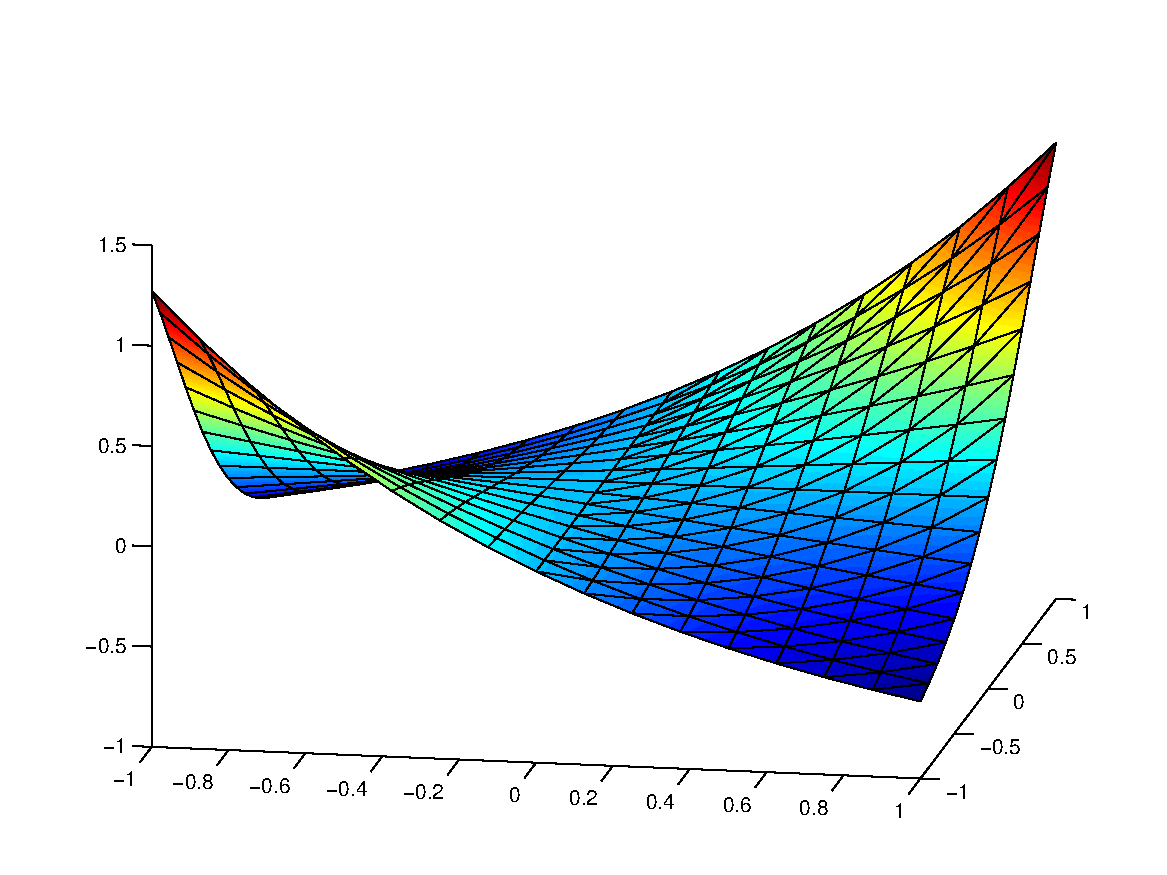
\includegraphics[height=0.27\textheight]{plots/poissonHybrid/phicubic16x16.pdf}\\
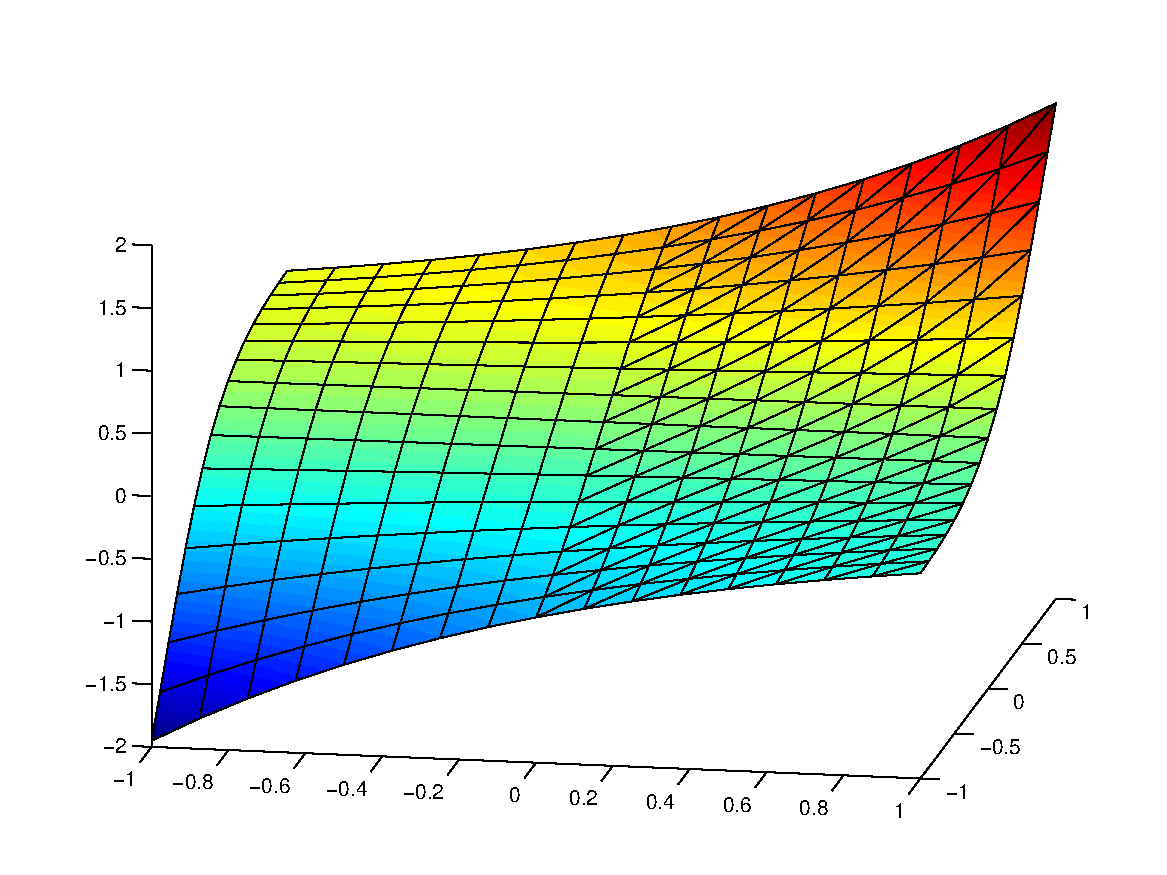
\includegraphics[height=0.27\textheight]{plots/poissonHybrid/psi1cubic16x16.pdf}\\
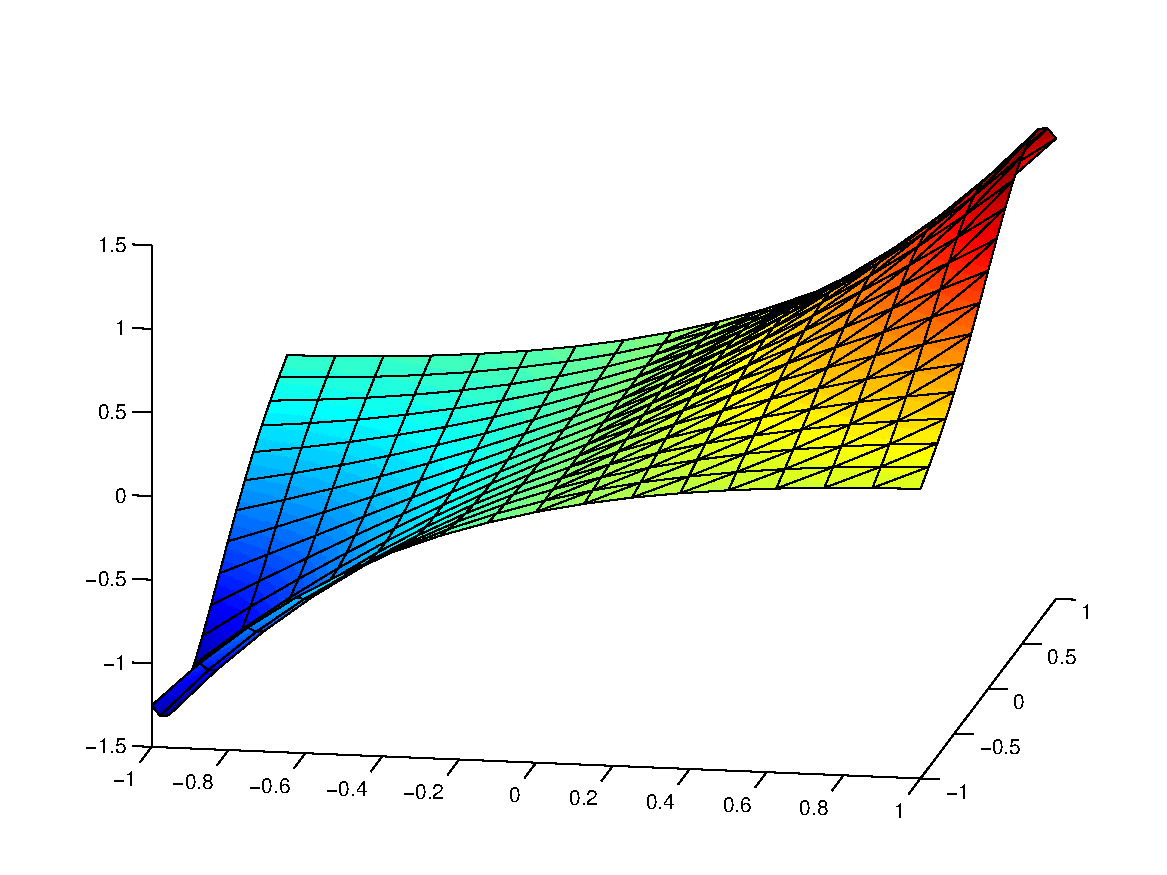
\includegraphics[height=0.27\textheight]{plots/poissonHybrid/psi2cubic16x16.pdf}
\caption{Solution of Poisson with quads and triangles (cubic elements, $16 \times 16$ mesh):
$\phi$ (top pane),
$\psi_{1}$ (middle pane)
$\psi_{2}$ (bottom pane).}
\label{NVR:fig:Poisson}
\end{center}\end{figure}

\begin{figure}[h!b!h!]
\begin{center}
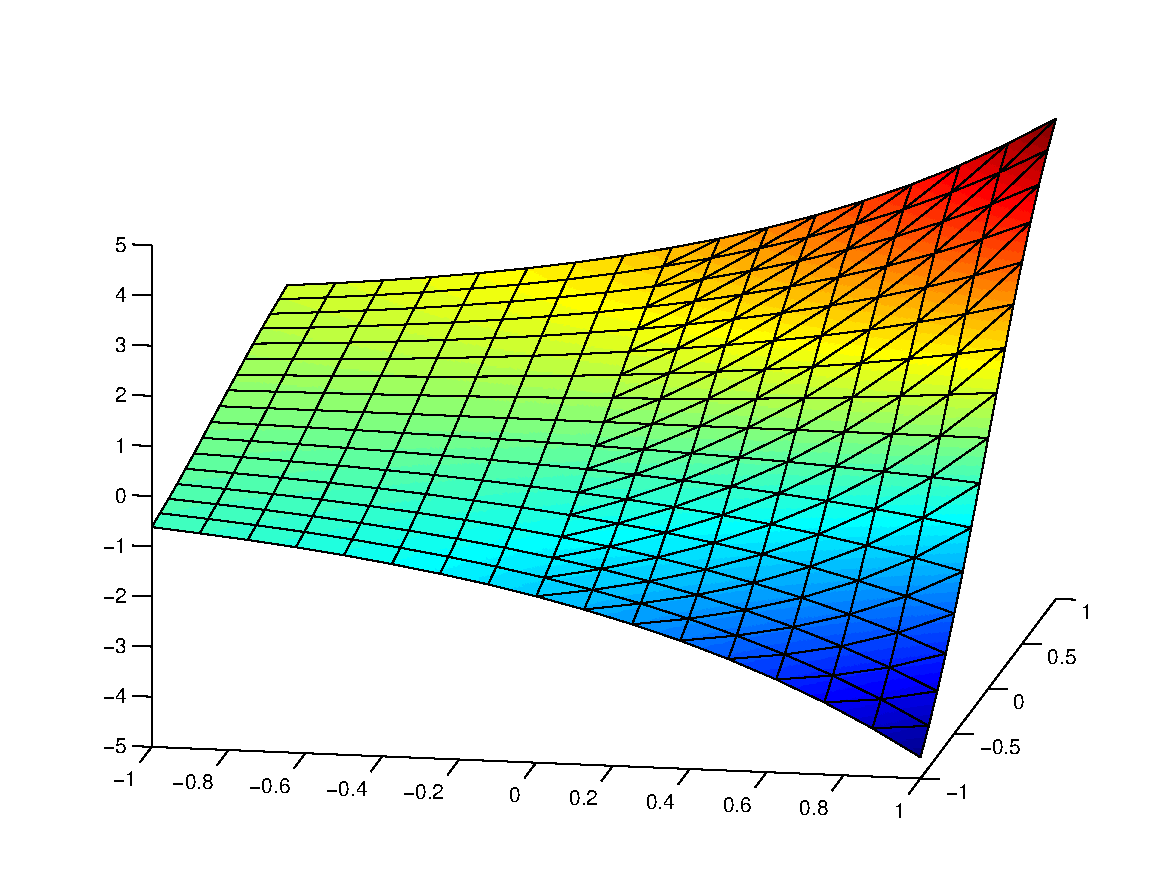
\includegraphics[height=0.27\textheight]{plots/stokesVVPHybrid/pressurecubic16x16.pdf}
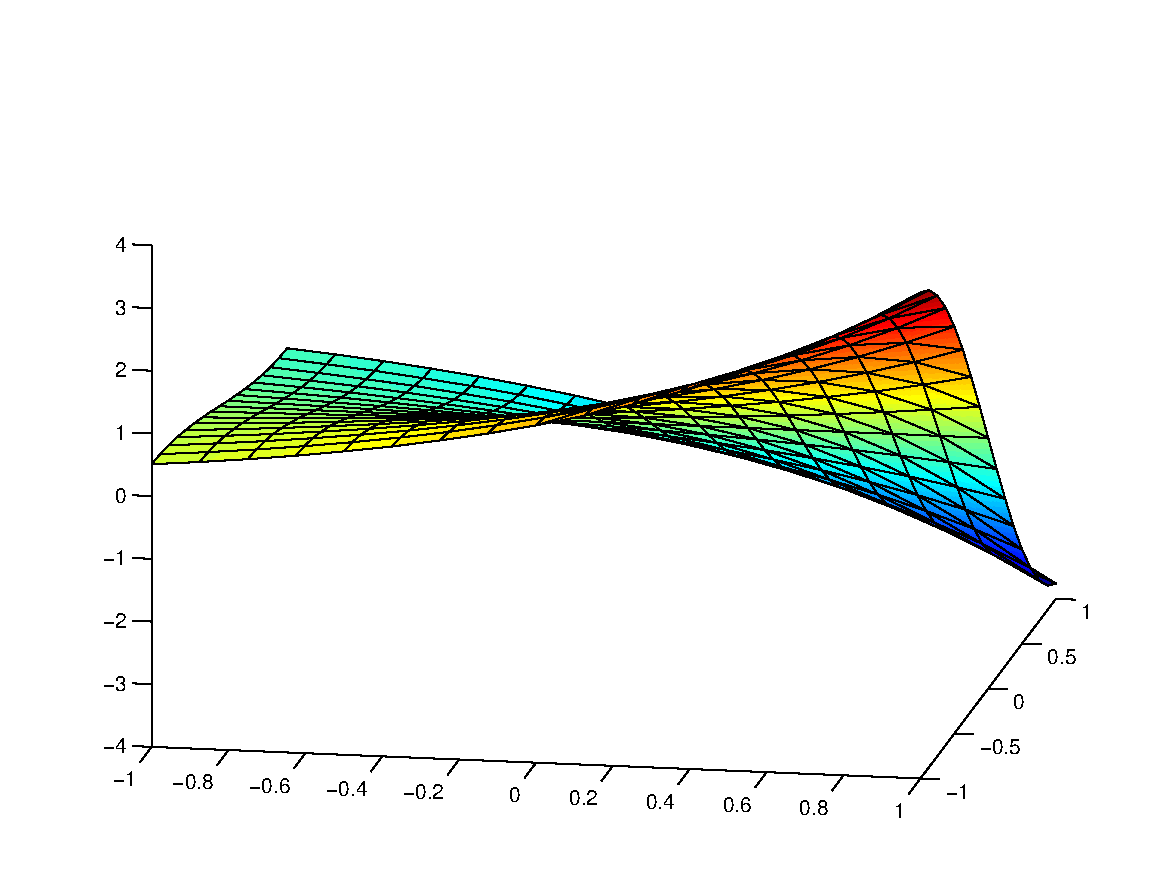
\includegraphics[height=0.27\textheight]{plots/stokesVVPHybrid/u1cubic16x16.pdf}
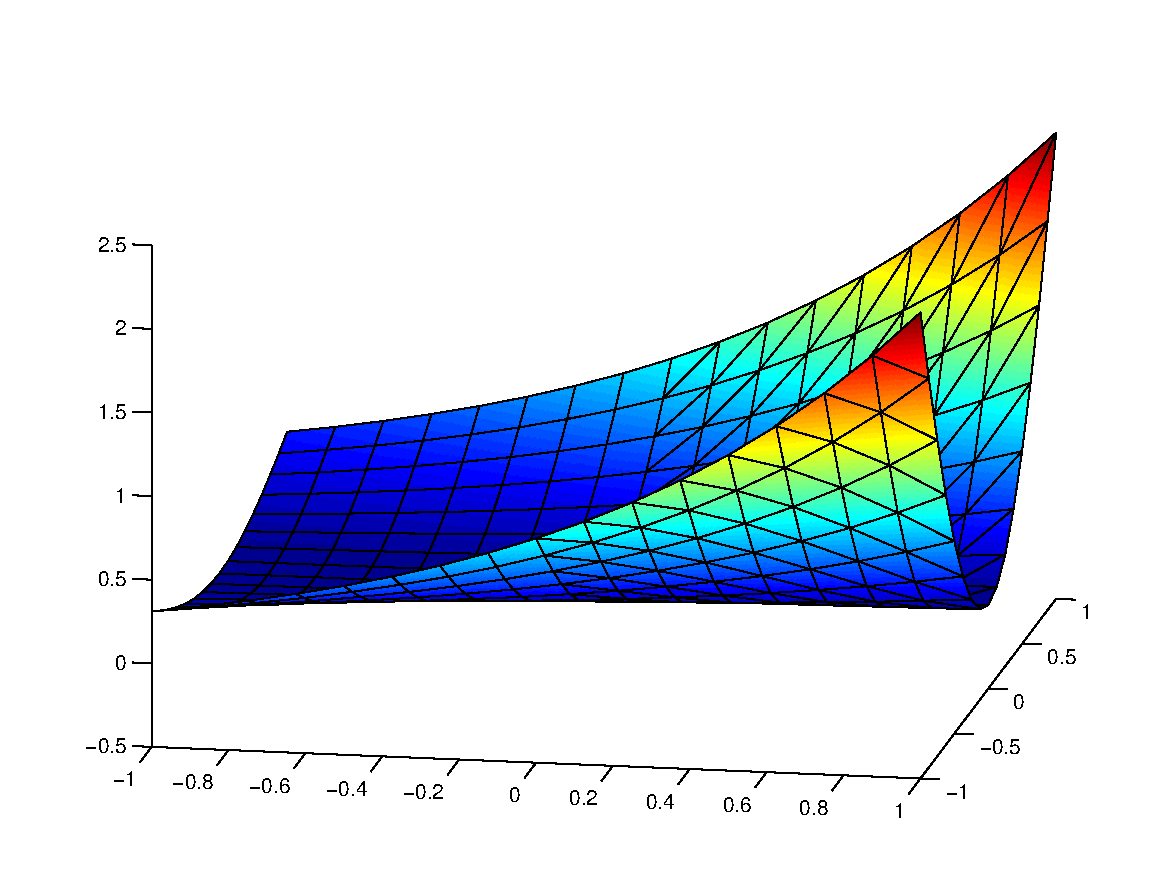
\includegraphics[height=0.27\textheight]{plots/stokesVVPHybrid/u2cubic16x16.pdf}
\caption{Solution of Stokes (VVP) with quads and triangles (cubic elements, $16 \times 16$ mesh):
$p$ (top pane),
$u_{1}$ (middle pane),
$u_{2}$ (bottom pane).}
\label{NVR:fig:Stokes}
\end{center}\end{figure}

\clearpage

\subsection{Extending Camellia for Distributed Stiffness Matrix Determination}\label{sec:distributingStiffness}
Here, we describe the changes that we implemented within Camellia to allow the stiffness matrix determination to be executed efficiently within an MPI environment.

Camellia was originally written to run in serial, so a number of changes were required to allow MPI execution---the most significant of these had to do with element partitioning and partitioning the degree-of-freedom coefficients.  Trilinos's Intrepid routines are designed to execute on batches of cells that are alike in topology and polynomial order.  We allow meshes of non-uniform topology and polynomial order; thus we had implemented an ElementType class which allowed us to identify elements that could be batched.  Our Mesh class maintained data structures such that information pertaining to a particular ElementType could be accessed quickly---for example, Mesh stored a data structure that contained the vertex coordinates belonging to elements of a given ElementType.

The upshot of this design is that mesh information is already, in a sense, partitioned.  However, there is no reason to expect that this will be a good partitioning for dividing up the work of stiffness matrix computation across MPI nodes---for this, we want our mesh partitioning to keep spatially adjacent elements together within a partition to minimize the amount of data that needs to be communicated during global stiffness matrix assembly.

Thus, to maintain both of our desired design features---batching by ElementType and spatially contiguous partitioning across MPI nodes---we require a two-level partitioning; we first divide the elements spatially (the MPI partitions), and then batch together elements of like ElementType within each of these partitions.  (Unfortunately, this is not quite the whole story; because other classes depend on the ElementType division of the whole mesh, we have had to maintain the old lookup tables as well.  We do hope to eliminate these dependencies in the end.)

To facilitate experiments with multiple partitioning strategies (and to maintain separation of concerns), we designed an abstract MeshPartitionPolicy class which, given a Mesh and the number of partitions desired, returns a partition of the elements in the mesh.  The Mesh then uses this to generate a partition of the degree-of-freedom coefficients, which induces a partition of the rows in the stiffness matrix.  The latter partition is used in conjunction with an Epetra FECrsMatrix, a distributed stiffness matrix class within Trilinos.  The FECrsMatrix allows storage of data not owned by the current MPI node; this data is communicated to the owning MPI node during global assembly of the stiffness matrix.  A convenient consequence of this is that we can separate the cost of global assembly from the cost of local stiffness matrix computations; the latter are independent across MPI nodes, and therefore we expect to see perfect scaling for these.  The scaling of the global assembly will depend on the quality of the partition and the cost of communication between MPI nodes.  We do not hope for perfect scaling here, but we do hope to see a cost per degree of freedom per node that does not grow too quickly in the total number of nodes.

The MeshPartitionPolicy partitions the mesh into sets of elements assigned to an MPI node; for the interface to Epetra, we need a partition of rows of the global stiffness matrix (each of which corresponds to a degree of freedom).  Degrees of freedom corresponding to numerical fluxes are shared by the elements along whose boundaries they lie.  We adopt a simple greedy policy for assignment of these d.o.f.s: shared d.o.f.s are assigned to the element with the smallest global identifier.  This means that even if the element partitioning were perfectly balanced, some MPI nodes might still have more d.o.f.s assigned to them than others.  This will not affect the amount of work involved in local stiffness matrix computations, but it may affect MPI communication costs during global assembly.

\paragraph{Design Limitations: where Amdahl's law might come to haunt us.}
Here, we note a few features of the present design that may become bottlenecks as we scale up to larger problems and larger numbers of MPI nodes.

At present, our global solve is implemented using the KLU implementation provided by the Amesos package within Trilinos.  This is a direct solve, executed in serial.  Amesos gathers the global stiffness matrix to rank 0, solves, and then scatters the solution according to the partition we have defined.  For our serial computations prior to the present work, the cost of the global solve has been dominated by the cost of the local optimal test function determination; however, now that the latter cost has been distributed using MPI and the former has not, we expect the global solve to become a bottleneck, both in terms of overall execution time and in terms of the sizes of problems that can be solved, since the KLU solve must fit into a single node's memory to be practical.

Similarly, at present the entire mesh is determined and stored on every MPI node.  This has the advantage that no MPI communication is required during mesh construction, but for very large meshes it may become impractical, because the time cost of mesh construction may grow relative to the distributed parts of the computation, and perhaps (for \emph{extremely} large meshes) because the memory required for the mesh may grow too large for storage on a node.

Finally, certain features of the original code depend upon all the solution coefficients being available to the current processor, so for the time being we distribute the entire solution to every MPI node, after Amesos has scattered according to the original partitioning.  We hope to eliminate this dependence on having all solution coefficients available, allowing the solution to be distributed according to the same mapping as was used for the stiffness matrix.

\subsubsection{Partitioning}

Since Camellia is tightly integrated with the Trilinos library already, we use the Zoltan package in Trilinos to generate spatially local partitions of the mesh \cite{ZoltanOverviewArticle}. We interface specifically with the Hilbert Space-filling Curve and Reftree partitioning algorithms in Zoltan, both of which can include parallel implementations. 

The Hilbert space-filling curve (HSFC) algorithm works by drawing a curve through the geometric mesh in 2- or 3-dimensional space, then mapping that curve to the interval $[0,1]$. The partitioner then divides up this interval (in an even or weighted manner) into $n$ partitions, and uses this partitioning to induce a partition of the mesh. All that's required by the HSFC algorithm is a listing of elements and a geometric identifier associated with a given element. In this case, we use the element centroid as such an identifier. 

The Reftree algorithm \cite{REFTREE} adds complexity in that each processor must store information not only about the active nodes, but the ancestors as well. Reftree also requires that if you store an ancestor, you also store all its children as well, increasing the amount of redundancy between distributed refinement trees. However, since Reftree is not tuned to a particular element types (quad or triangle, tetrahedron or cube), the same algorithm performs similarly for many different types of refined meshes (as opposed to HSFC, which works best for quadrilateral grids, but not for triangular grids).  Additionally, Reftree's algorithm guarantees connected partitions for tetrahedral and triangular grids, and generally performs more robustly on other types of grids as well.

Currently, we have implemented and tested a Reftree MeshPartitionPolicy on our workstations. However, Reftree currently crashes during runs on Lonestar, our HPC architecture for this report. We used the HSFC partitioner for the scaling tests in this report, and hope to fix issues with Reftree in the near future. 

\subsubsection{Scaling tests}\label{sec:ScalingExperiments}

We tested the scalability of our code on the Lonestar machine at the Texas Advanced Computing Center (TACC), verifying whether or not we observe strong/weak scaling for various parts of the program.  We solve the convection-diffusion equation on a square mesh, with boundary conditions such that the solution develops a boundary layer (sharp gradient) near the north and east edges of the square.  The solution for a refined mesh is shown in Figure \ref{fig:solutionPlot}.

\begin{figure}[h!]
\centering
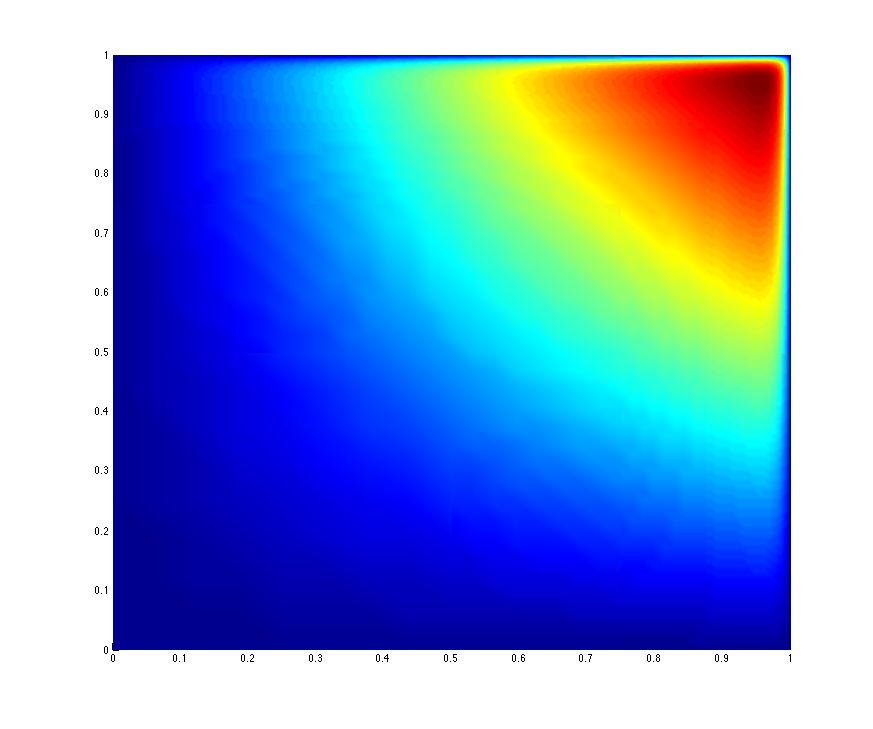
\includegraphics[scale=0.45]{figs/Solution12928nomesh.png}
\caption{Computed solution for $\epsilon=10^{-2}$ using a 12,928-element mesh.  $L^2$ error is $O(10^{-5})$.}
\label{fig:solutionPlot}
\end{figure}

We set up our computational experiments by first refining all cells that share an edge with the north and east sides, and repeating this process four times.   We then constructed three additional meshes, by uniformly refining every element in the mesh (quadrupling the number of elements each time).  For each of these meshes, we solved on Lonestar, using 1, 4, 16, and 64 nodes, tracking the timing of various portions of the code.  From this data, we extracted strong and weak scaling statistics, discussed below in Sections \ref{sec:strongScaling} and \ref{sec:weakScaling}.  The runtimes plotted in each of our figures are the mean of the times recorded at each MPI node.

We also used contiguous and discontiguous partitions of each mesh to measure the effect of partition quality on the communication costs in global stiffness matrix assembly.  We created contiguous partitions of the mesh using a HSFC partitioner.  To create the discontiguous partitioning, we used the Zoltan cyclic partitioner, which loops through the list of active elements, sending the first element to the first processor, the next to the next processor, and so on.  After reaching the last processor, the cyclic partitioner cycles back to the first processor and repeats this process.\footnote{Due to the nature of our refinements in this test, a blocked partitioner (equally partitioning the ordered list of active elements by element number) happened to produce nearly-contiguous partitions.  We therefore have omitted this partitioner from our analysis, since we do not believe that its performance here accurately predicts its performance in general.}  The cyclic partitioning is a ``worst case" scenario in the sense that each of the current MPI node's elements' neighbors are owned by some other MPI node, with the consequence that information concerning each element boundary must be sent via MPI.  An example cyclic partitioning can be seen in Figure \ref{fig:cyclicPartition}; Figure \ref{fig:HSFCPartition} shows an HSFC partitioning.

It's worth noting that the runtimes reported here do not represent Camellia running at peak efficiency.  A single Lonestar node contains 12 cores.  Because MPI communication has much higher bandwidth intra-node than inter-node, and for analysis we wanted approximately equal bandwidth between MPI processes, we use only one core per node.  Utilizing all 12 cores on a node would decrease communication costs.  Additionally, there is a parameter within Camellia that controls the batch size for the Trilinos Intrepid batching routines.  Tuning this parameter based on machine-specific cache sizes should further improve performance.

\begin{figure}[h!]
\centering
\subfigure[Cyclic partitioning]{\label{fig:cyclicPartition}
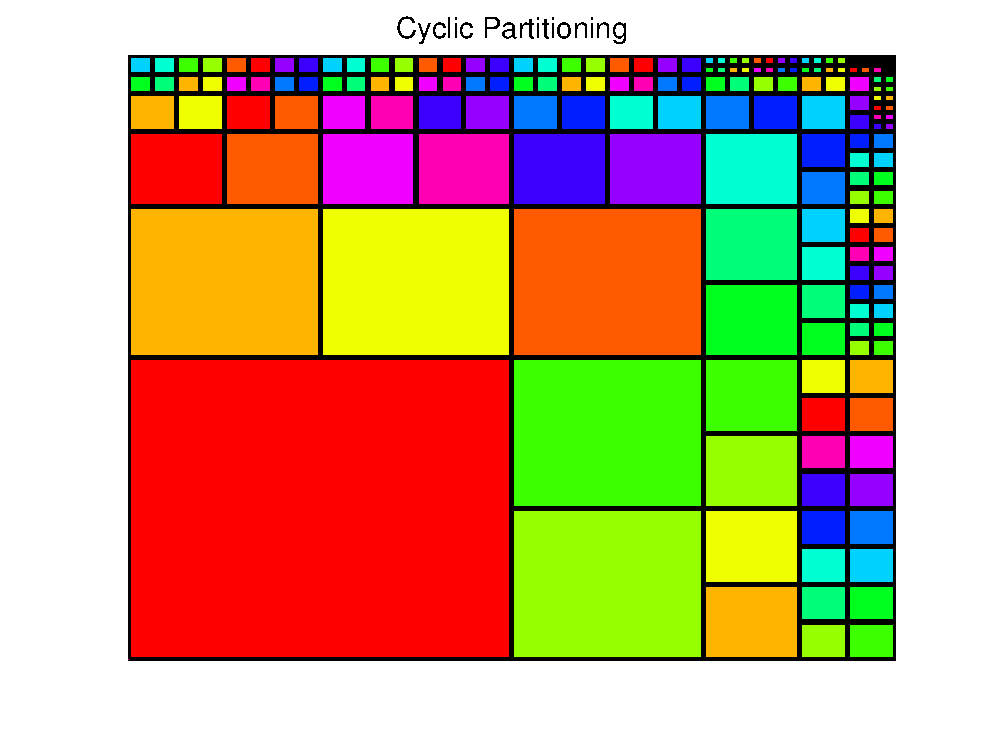
\includegraphics[scale = 0.42]{figs/cyclic.pdf}
}
\subfigure[HSFC partitioning]{\label{fig:HSFCPartition}
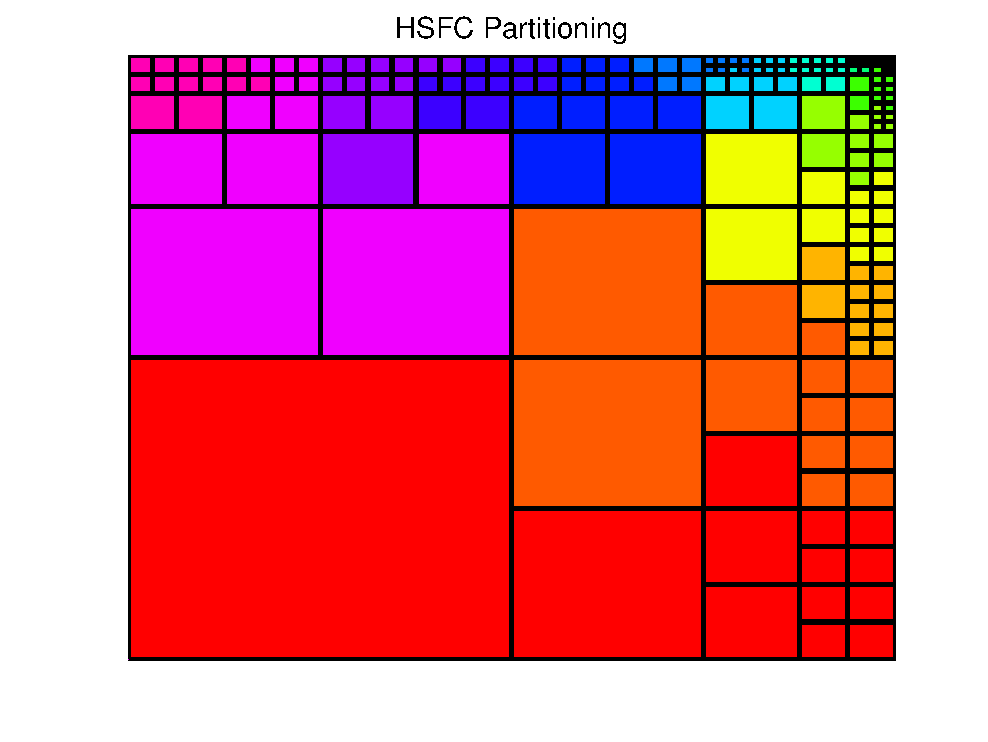
\includegraphics[scale = 0.42]{figs/hsfc.pdf}
}
\caption{Discontiguous and contiguous partitions of the mesh.}
\end{figure}

\subsubsection{Strong scaling}\label{sec:strongScaling}
In our strong scaling tests, we considered problems of fixed size, distributing the workload for each among increasing numbers of MPI nodes.  Here, we hope to see runtimes that decrease linearly in the number of MPI nodes---this is what we mean by achieving strong scalability.

Because the local stiffness computations are entirely independent of each other, requiring no communication among MPI nodes, we expect to see perfect scaling for these.  As can be seen in Figures \ref{fig:strongScalingLocalStiffnessCyclic} and \ref{fig:strongScalingLocalStiffnessHSFC}, we do achieve something very close to this, although the cyclic partitioning took longer in almost every case, for reasons that are unclear to us.  It may have something to do with data locality on each node---by the manner of our construction, data concerning contiguous mesh elements is more likely to be close together in memory than the data for mesh elements in the cyclic case.

It is less clear what we should expect for the global stiffness matrix assembly; we expect the HSFC partitioning to outperform the cyclic partitioning, and we would like to see the runtimes for assembly decrease as the number of MPI nodes increases.  As can be seen in Figures \ref{fig:strongScalingAssemblyCyclic} and \ref{fig:strongScalingAssemblyHSFC}, for the larger problems in both cases, we do have something approaching strong scalability.  For the 202- and 808-element problems, we see the time cost increase (or fail to decrease, in the case of the 808-element problem for the cyclic partitioner) between 16 and 64 nodes.  However, it's worth noting that in these cases, the real times involved are small: less than a second in each case.  If our concern is our ability to scale up to large problems on large numbers of processors, it does not appear that the global assembly will be a bottleneck.  The HSFC partitioning does show its strength here compared with the cyclic; for the 12,928 mesh on the 4-node run, the cyclic partitioning took an average of 49.1 seconds per node, compared with 1.63 seconds for the HSFC partitioning.

\begin{figure}[h!]
\centering
\subfigure[Cyclic Partitioning]{\label{fig:strongScalingLocalStiffnessCyclic}
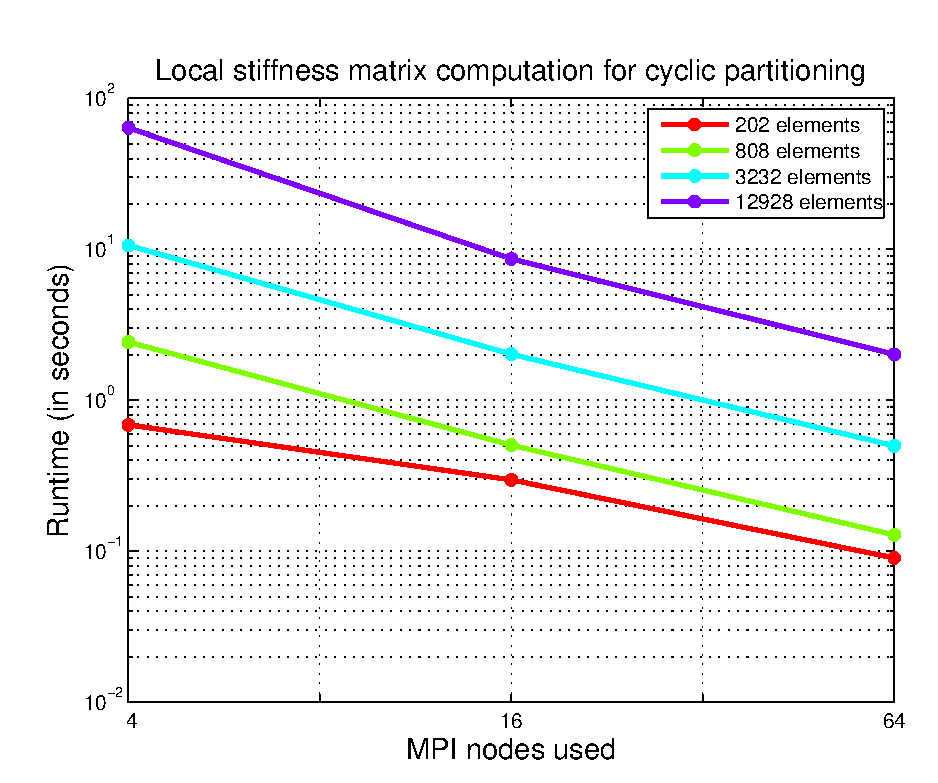
\includegraphics[scale = 0.42]{figs/scalingFigs/cyclicStrongScalingLocal.pdf}
}
\subfigure[HSFC Partitioning]{\label{fig:strongScalingLocalStiffnessHSFC}
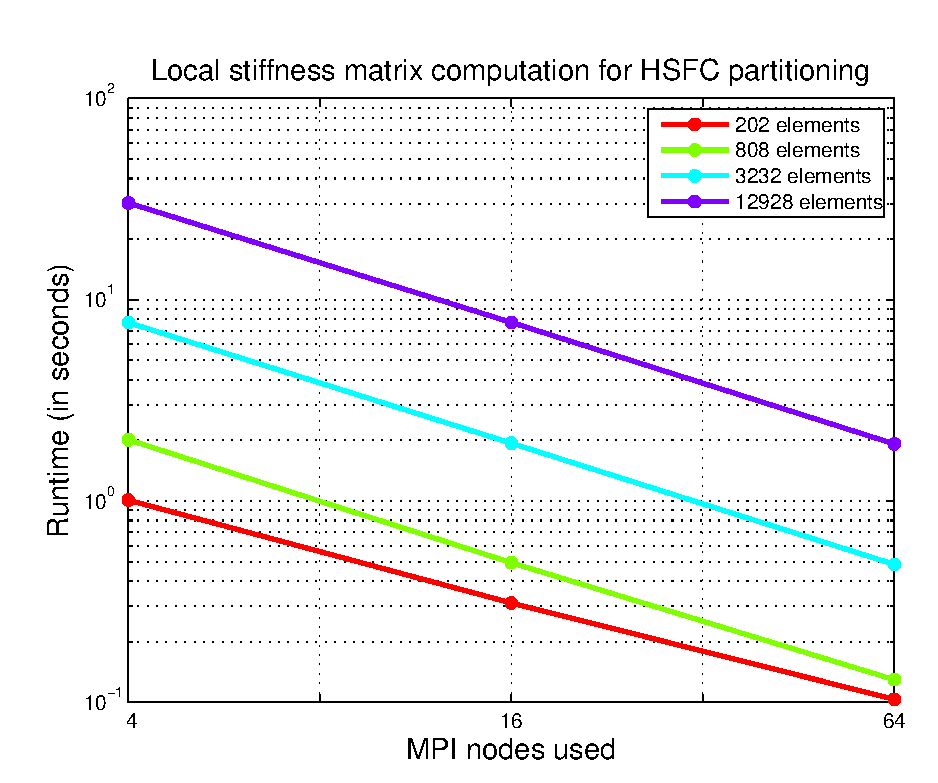
\includegraphics[scale = 0.42]{figs/scalingFigs/hsfcStrongScalingLocal.pdf}
}
\caption{Strong scaling plots for the local stiffness matrix computation.}
\end{figure}

\begin{figure}[h!]
\centering
\subfigure[Cyclic Partitioning]{\label{fig:strongScalingAssemblyCyclic}
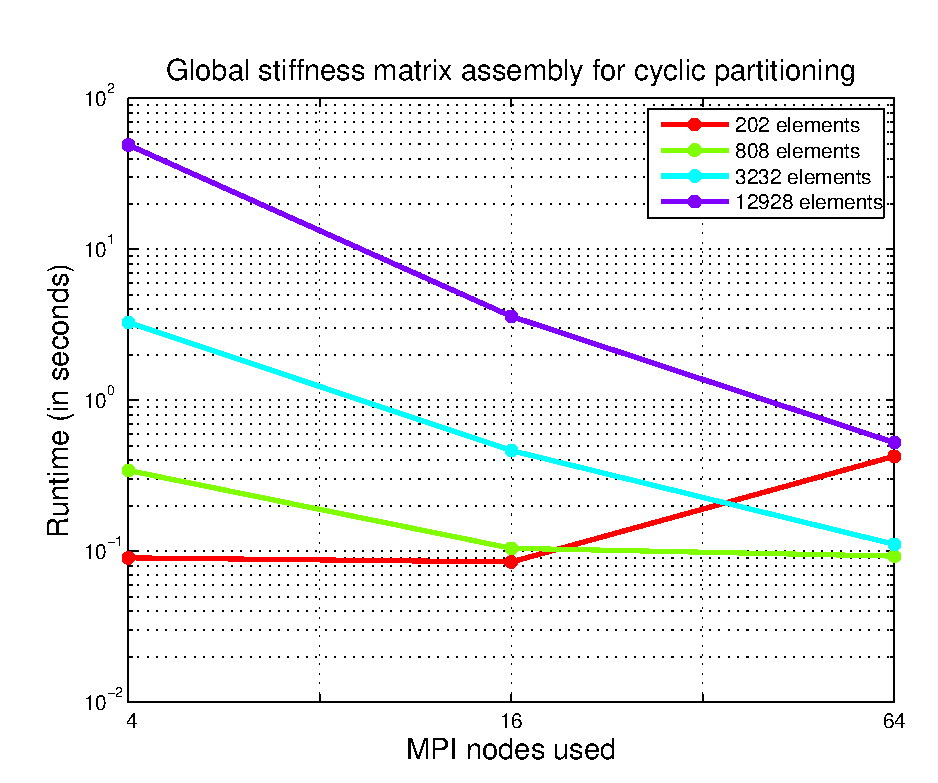
\includegraphics[scale = 0.42]{figs/scalingFigs/cyclicStrongScalingAssembly.pdf}
}
\subfigure[HSFC Partitioning]{\label{fig:strongScalingAssemblyHSFC}
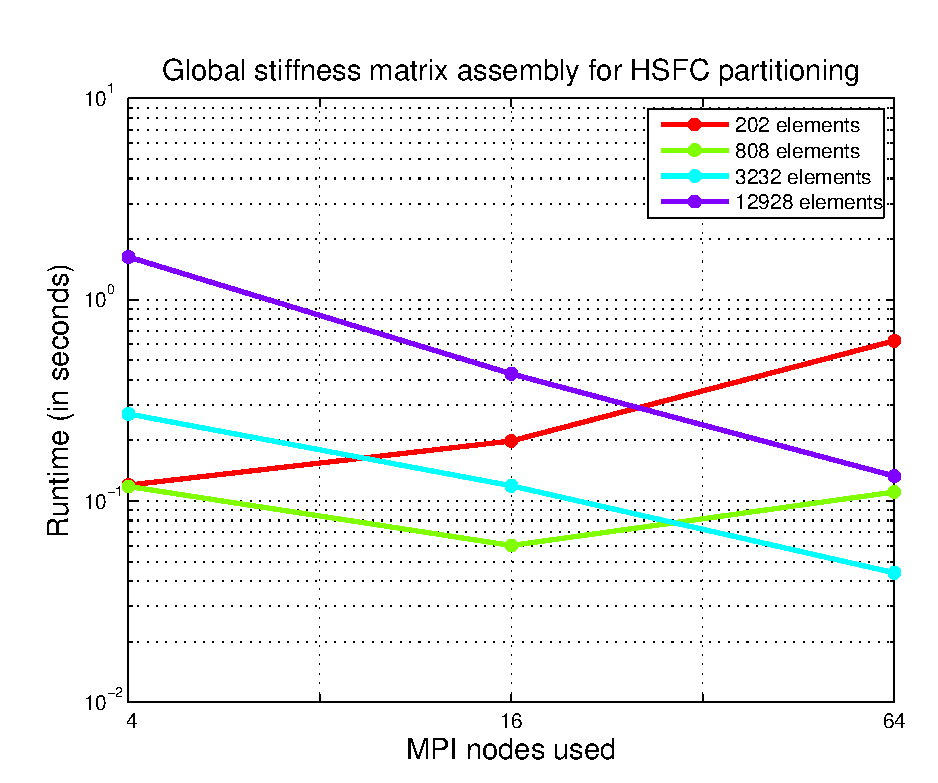
\includegraphics[scale = 0.42]{figs/scalingFigs/hsfcStrongScalingAssembly.pdf}
}
\caption{Strong scaling plots for global stiffness matrix assembly.  (Note the differing scales.) }
\end{figure}

\subsubsection{Weak scaling}\label{sec:weakScaling}
In our weak scaling tests, we aimed to fix the size of the problem \emph{per MPI node}, and examined the runtime of various portions of the execution---we hope to see a constant runtime as the problem size and number of processors increase, and this is what we mean by achieving weak scalability.

\begin{figure}[h!]
\centering
\subfigure[Local stiffness computation]{
\label{fig:weakScalingStiffness}
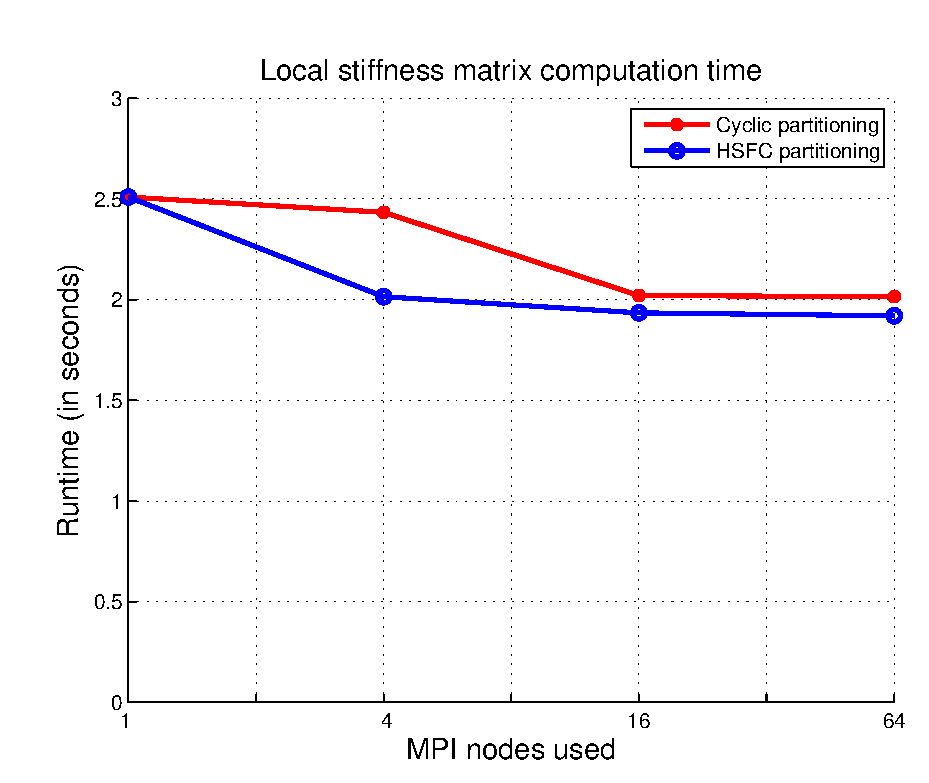
\includegraphics[scale = 0.42]{figs/scalingFigs/weakScalingLocal.pdf}
}
\subfigure[Global stiffness assembly]{
\label{fig:weakScalingAssembly}
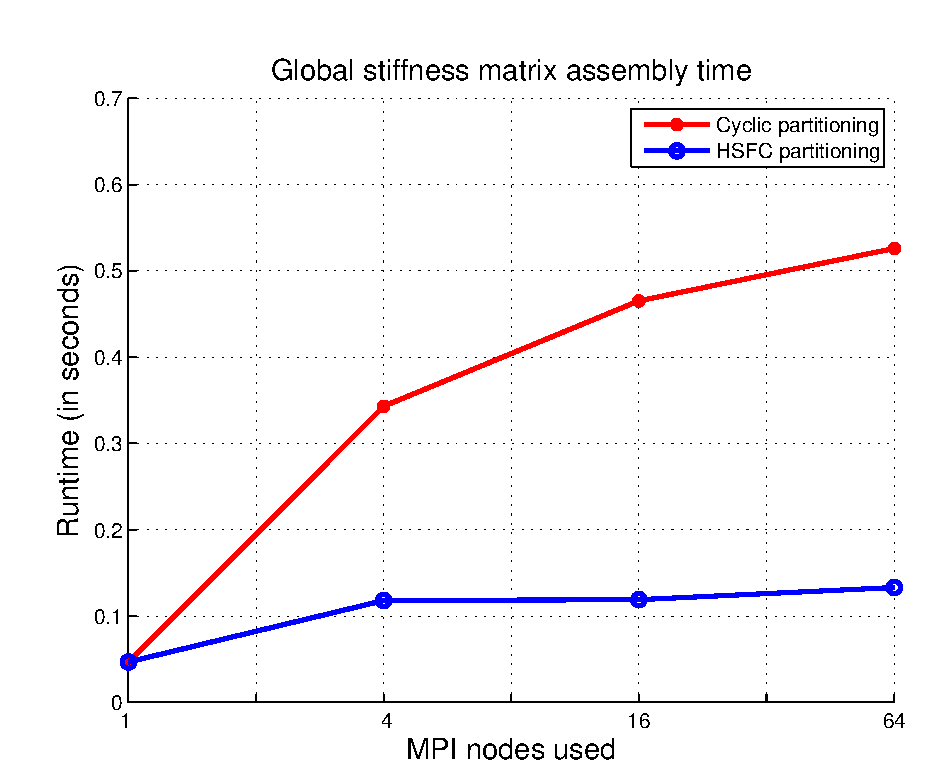
\includegraphics[scale = 0.42]{figs/scalingFigs/weakScalingAssembly.pdf}
}
\caption{Weak scaling results for computation of local stiffness matrices and global stiffness matrix assembly.  For each run, both the number of MPI nodes and the number of elements increased by a factor of four.}
\end{figure}

Both partition types achieve weak scalability in the local stiffness matrix computation, as can be seen in Figure \ref{fig:weakScalingStiffness}.  In fact, we see the total runtime \emph{decrease} slightly as the total workload and number of MPI nodes increase---we are unsure of the reason for this. Although we would not expect the partitioning to affect this portion of the computation at all (since no inter-node communication occurs at this stage), for some reason the HSFC partitioning slightly outperforms the cyclic on each of the multi-node runs.  As with the strong scaling, we speculate that this is due to locality of the owned element data in the case of the HSFC partitioning.

Assembly of the global stiffness matrix achieves weak scalability only for the contiguous case, as can be seen in Figure \ref{fig:weakScalingAssembly}. It's worth noting, however, that though the poor mesh partitioning imposes much higher communication costs than the HSFC partitioning, the maximum amount of time spent on assembly is still dominated by the time spent on computation of local stiffness matrices.

\subsubsection{Total runtime analysis}\label{sec:runtimeAnalysis}
As the final component of our performance analysis, we examine components of the total runtime for each of our four problems using 1, 4, 16, and 64 MPI nodes; here we use the HSFC partitioner.  This can be seen in Figure \ref{fig:timeBreakdown}.  We see that for the largest MPI runs the combined time spent on local stiffness computation and global assembly is a small fraction of the total time spent---since these were the targets of the present work, we can count it a success.  The graphs also show that the cost of the global solve dominates in each of these runs, making this the obvious next target for optimization.  In the ``Other'' category, the largest cost is the mesh determination.  In the 12,928-element case, this takes about 5 seconds.  Thus, a distributed mesh might be our next target after the solve is optimized.

\begin{figure}[h!]
\centering
\subfigure[202 elements, 13,343 dofs]{
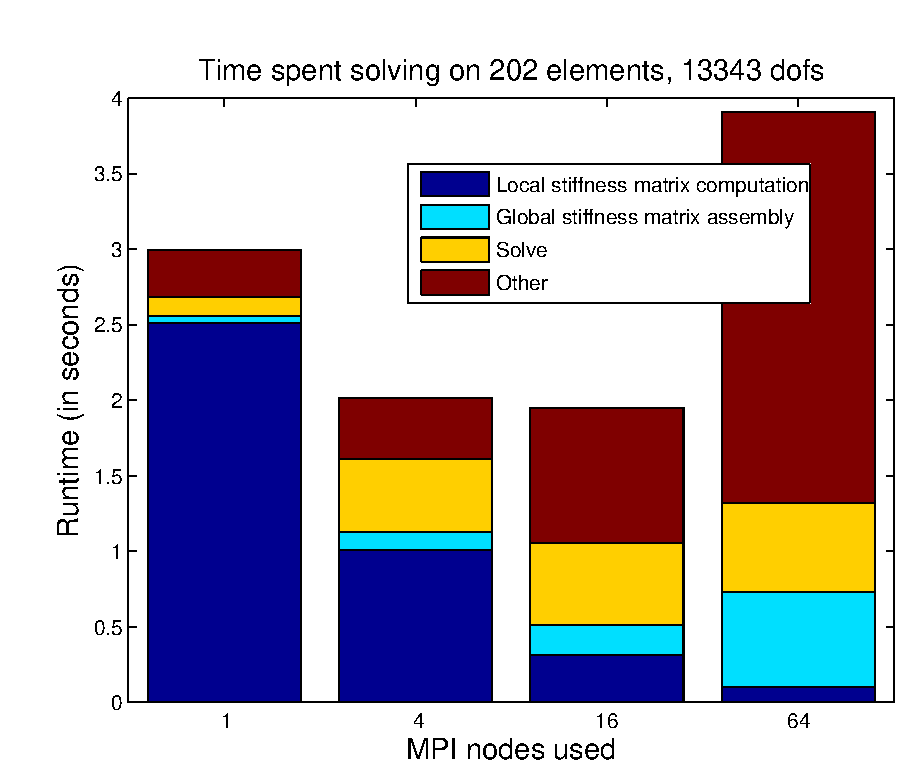
\includegraphics[scale = 0.42]{figs/scalingFigs/bar_ref0.pdf}
}
\subfigure[808 elements, 52,137 dofs ]{
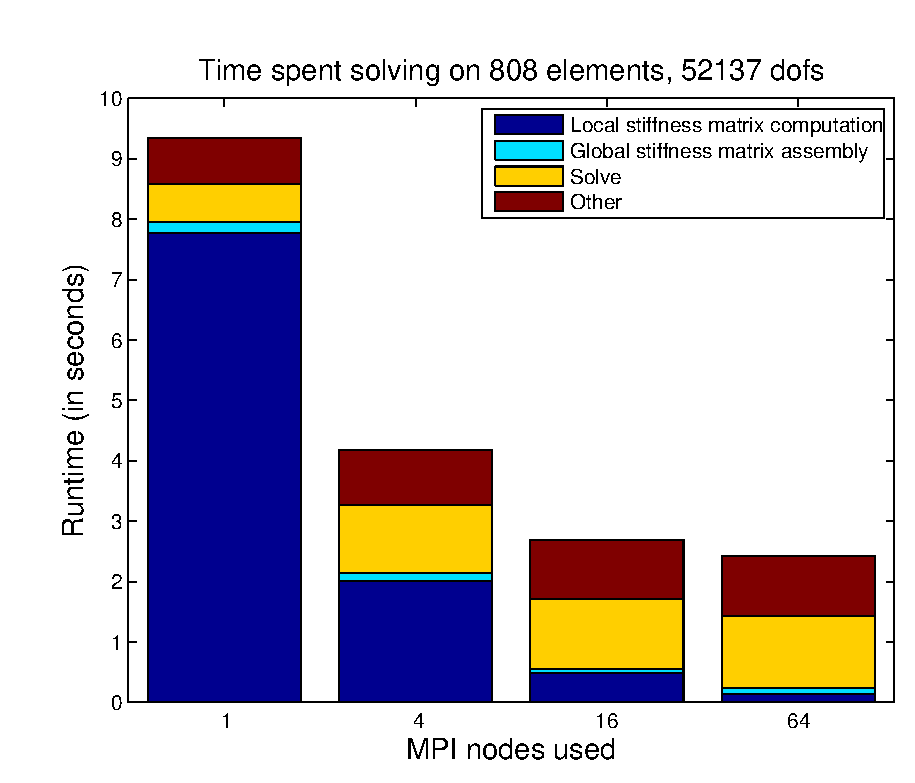
\includegraphics[scale = 0.42]{figs/scalingFigs/bar_ref1.pdf}
}
\subfigure[3,232 elements, 206,081 dofs]{
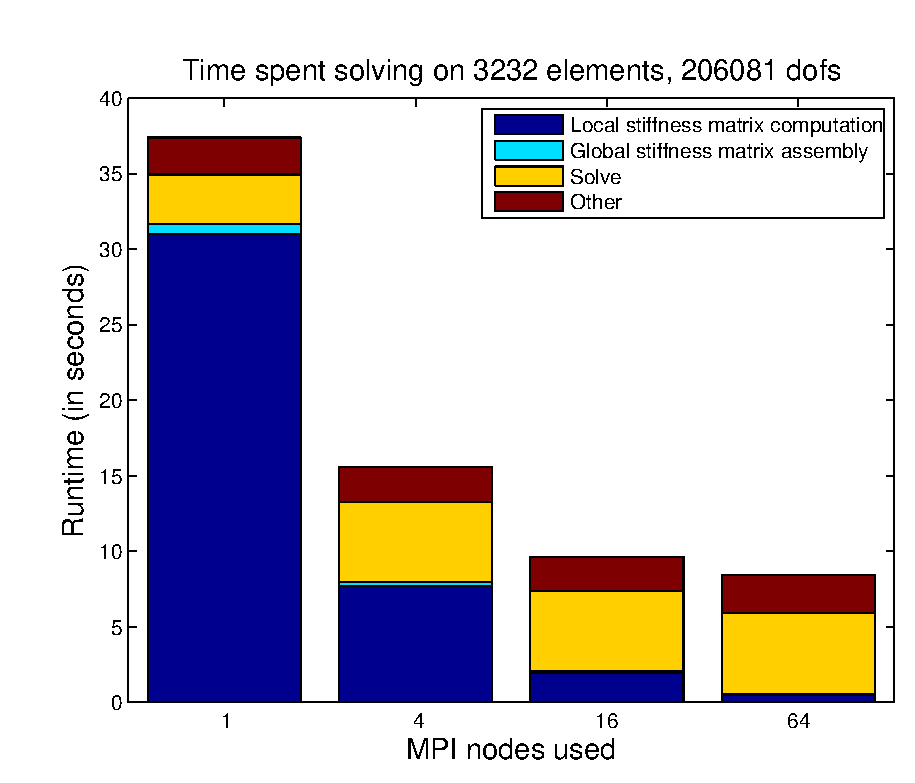
\includegraphics[scale = 0.42]{figs/scalingFigs/bar_ref2.pdf}
}
\subfigure[12,928 elements, 819,393 dofs]{
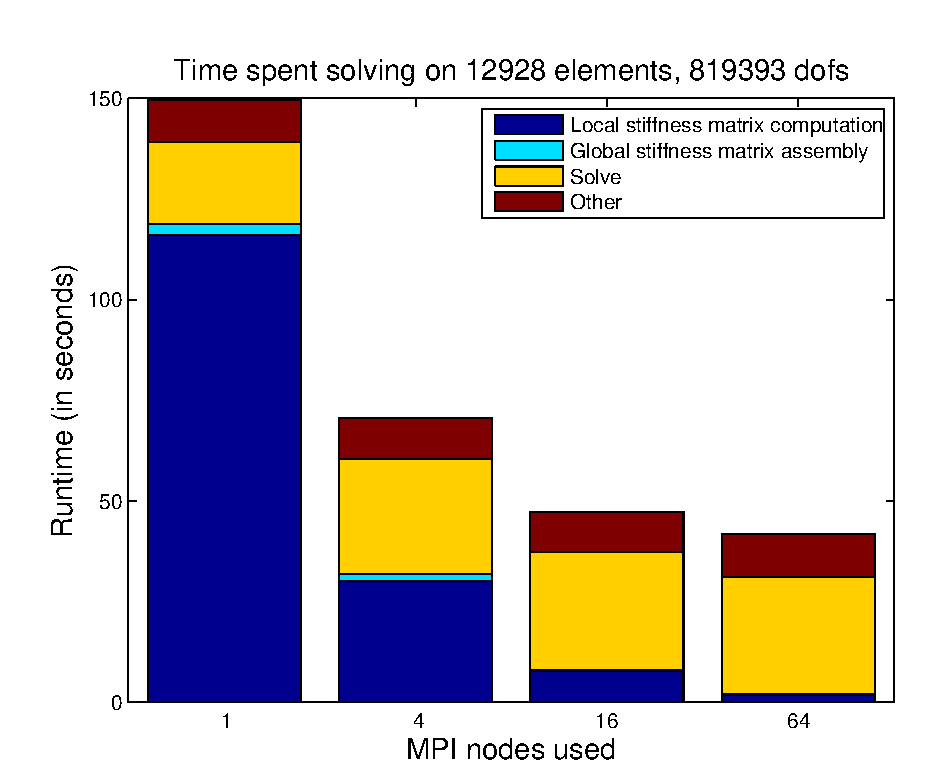
\includegraphics[scale = 0.42]{figs/scalingFigs/bar_ref3.pdf}
}
\caption{Breakdown of time spent in a solve for a series of HSFC-partitioned meshes.}
\label{fig:timeBreakdown}
\end{figure}

\subsubsection{Future Work for Better Scaling}\label{sec:FutureWork}
There are several ways in which we hope to extend Camellia further to allow it to solve larger problems still; we hope to:
\begin{itemize}
\item distribute the solve, using MUMPS or an iterative solver,
\item improve the load balancing for meshes of variable polynomial order,
\item distribute mesh construction and storage, and
\item distribute solution storage.
\end{itemize}

As discussed in Section \ref{sec:runtimeAnalysis} above, the lowest-hanging fruit for further improving the performance for the experimental setup considered in the present work is distributing the solve.  We have already successfully interfaced with MUMPS---a parallel sparse direct solver---on one of our laptops; we expect that getting MUMPS to work on Lonestar will just be a matter of building Trilinos and Camellia with MUMPS there.  One of the advantages of DPG is that its stiffness matrices are guaranteed to be symmetric positive definite, which opens the door to using iterative methods such as conjugate gradient methods.  DPG also produces matrices whose entries are coupled only through the flux degrees of freedom; thus static condensation techniques can be used to reduce the size of the global system to be solved.  We believe that iterative solvers and static condensation would allow us to solve larger problems than MUMPS will allow---we have heard that MUMPS only scales to about 128 processors.

In the present work, we considered a mesh of uniform polynomial order and considered all elements to be of equal weight; Camellia supports meshes with variable order, and Zoltan provides facilities for weighting elements differently.  By taking advantage of this feature of Zoltan (using a weight corresponding to the number of degrees of freedom on each element), we can improve Camellia's load balancing for meshes of variable polynomial order.  In fact, in doing so, we expect to improve slightly the load balancing for the setup considered here, because elements with hanging nodes do have slightly more degrees of freedom than those without.

At present, the mesh is constructed and stored on each node, as is the solution.  It should be a relatively small extension to the present work to allow the solution to be distributed.  Allowing mesh construction to be distributed is a bigger challenge, largely because the nodes must agree on the global stiffness matrix row indices.  Given that we are working with an adaptive mesh, it will likely make sense to distribute the work of mesh refinement according to the partition of the previous mesh and use Zoltan to do the load rebalancing.

In summary, we have achieved good overall speedup for Camellia using a Hilbert space-filling curve partitioner, and have identified the next steps for improving its parallel performance further.

\subsection{Demonstration of Nonlinear Solution Capabilities: Compressible Navier-Stokes}\label{sec:compressibleNS}
Jesse Chan has applied Camellia's nonlinear solve capabilities to the compressible Navier-Stokes equations in the context of Carter's flat plate problem.  We include here some plots that demonstrate the success of the adaptive mesh (Figure \ref{fig:JCmeshRefinements}), as well as a plot of the final solution for the velocity in the $x$ direction (Figure \ref{fig:JCu1}).  This experiment was performed with a Reynolds number of 1000 and a Mach number of 3.

\begin{figure}[h!]
\centering
\subfigure[i=0]{
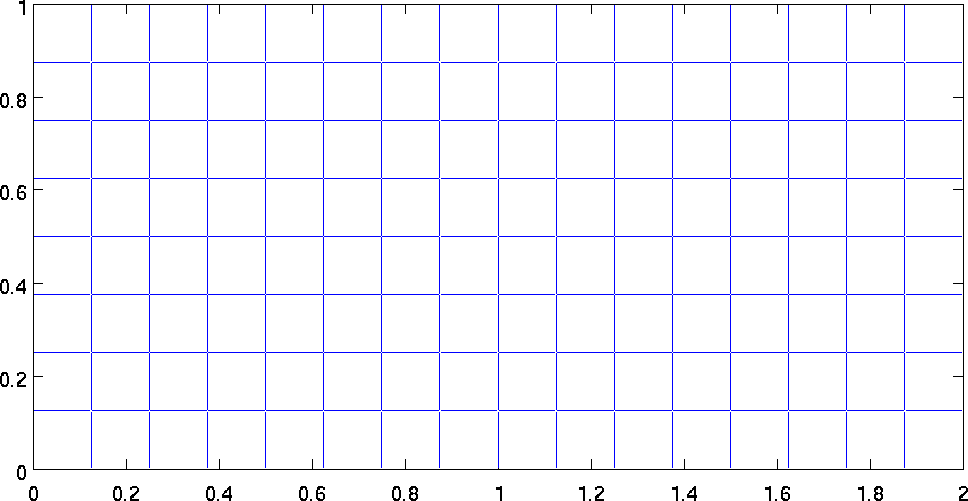
\includegraphics[scale = 0.45]{figures/mesh0.png}
}
\subfigure[i=1]{
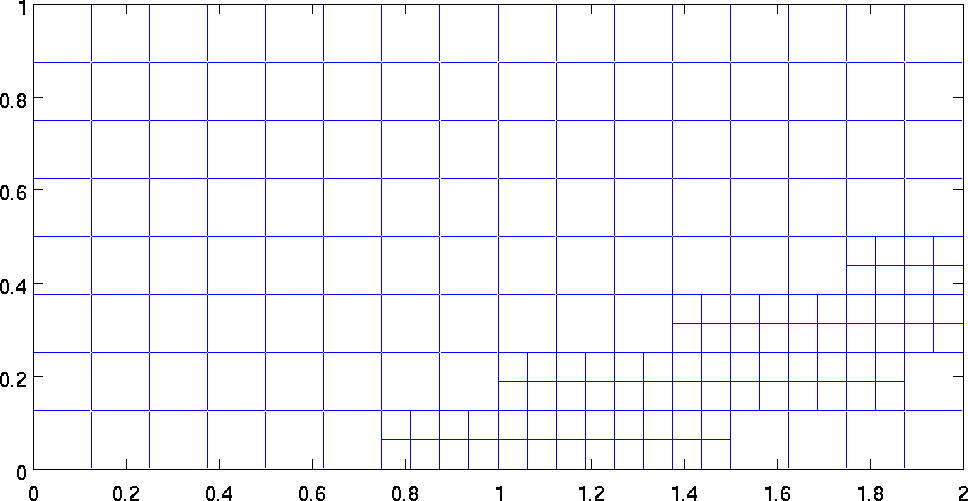
\includegraphics[scale = 0.45]{figures/mesh1.png}
}
\subfigure[i=2]{
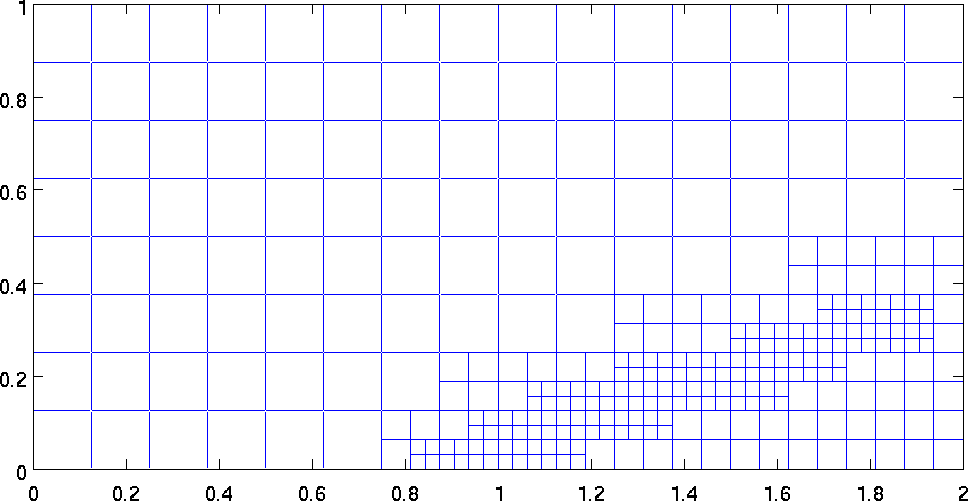
\includegraphics[scale = 0.45]{figures/mesh2.png}
}
\subfigure[i=4]{
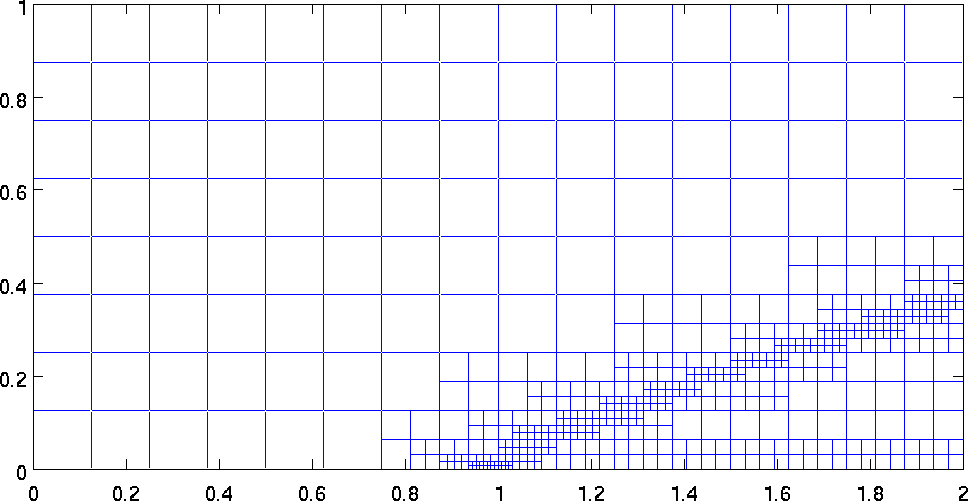
\includegraphics[scale = 0.45]{figures/mesh4.png}
}
\subfigure[i=5]{
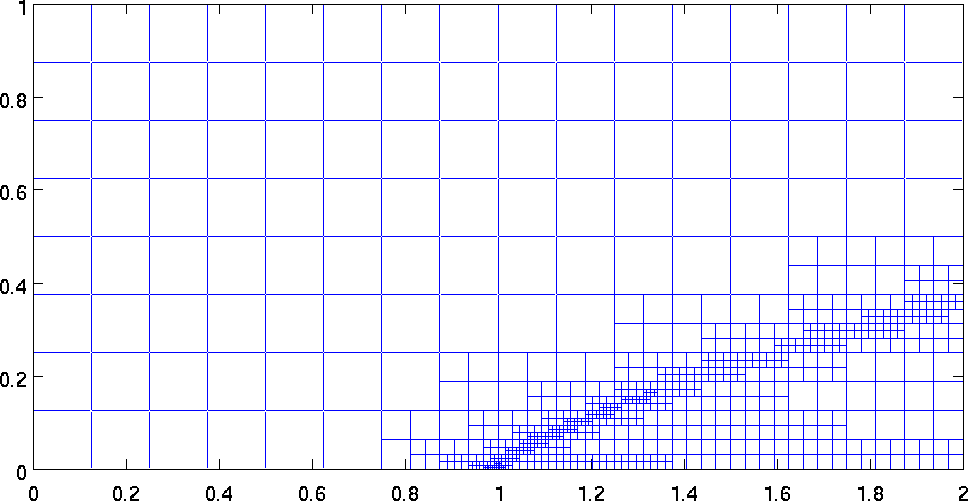
\includegraphics[scale = 0.45]{figures/mesh5.png}
}
\subfigure[i=6]{
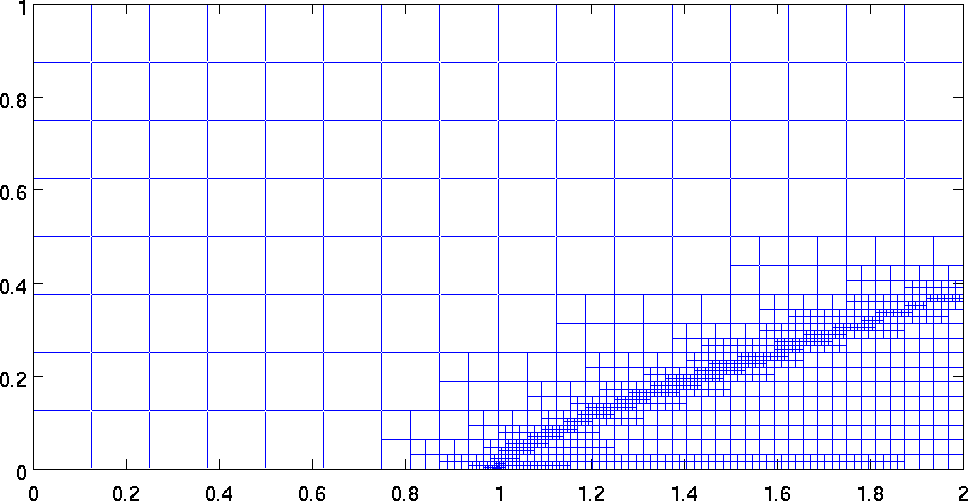
\includegraphics[scale = 0.45]{figures/mesh6.png}
}
\caption{Mesh refinements for compressible Navier-Stokes in Carter's flat plate problem.  The $i$ values are the refinement number (i.e. $i=0$ corresponds to the initial mesh).}
\label{fig:JCmeshRefinements}
\end{figure}

\begin{figure}[h!]
\centering
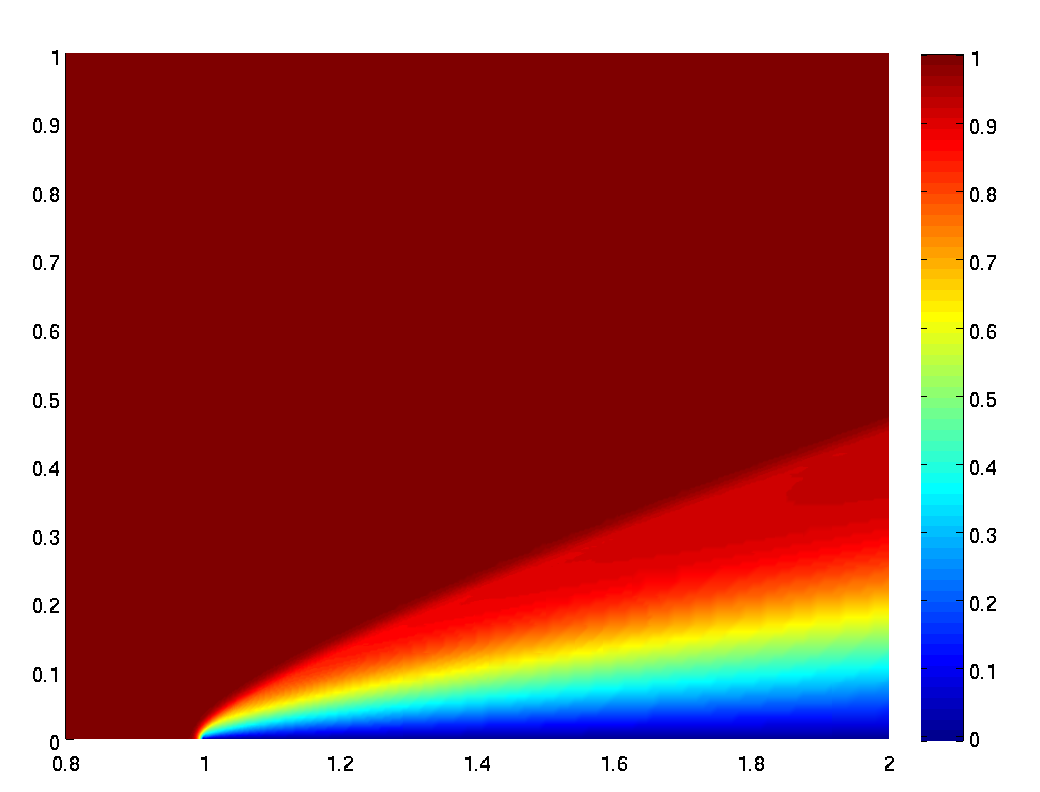
\includegraphics[scale = 0.90]{figures/u1.pdf}
\caption{Final solution for the $x$ component of the velocity in Carter's flat plate problem.}
\label{fig:JCu1}
\end{figure}

%\subsection{Meshing, Solving, and Adaptivity}\label{sec:Meshing}   both what's there now, and what we will eventually do.  This is where our idea for the $hp$-decision algorithm should go.
%\subsubsection{Handling Hanging Nodes: MultiBasis and PatchBasis}\label{sec:HangingNodes}
%\subsection{Nonlinear Problems}\label{sec:NonlinearProblems}
%\subsection{Comparison between Camellia and deal.II}\label{sec:Deal.II}
%\subsection{Summary}\label{sec:CamelliaConclusion}

\clearpage